\section{Prolusion --- Course Introduction}\label{sec:prolusion}

This is the opening lecture of \textbf{Advanced Statistical Learning and Modeling}, taught by Prof. Roberta Siciliano at DIETI, University of Naples Federico II. It is an introductory, organizational lecture: no exam-relevant formulas here, just the map of what the course is about and how it is run.

\subsection{Welcome, motivation, and the Stad Lab team}\label{sec:prolusion-welcome}

\subsubsection{An opening quote}

The lecture opens with a quote by George Henry Lewes (1877): \textit{``Science is the systematic classification of experience.''} The idea behind it: science is not about collecting facts randomly, but about organizing observations into a coherent structure that lets us understand and predict. This is exactly what statistics and machine learning try to do with data.

\subsubsection{Agenda of the prolusion}

The lecture is organized into five parts:
\begin{itemize}
  \item The human side of science: the \textbf{Stad open lab} research group.
  \item Raw data and the \textbf{Stad methodological pipeline}.
  \item The probabilistic perspective of the machine learning paradigm (covered in the next chunk).
  \item Statistical learning theory and foundations (covered later).
  \item Textbooks and exam information (covered later).
\end{itemize}

\subsubsection{The human side of science}

Before diving into methods, the course stresses a simple point: data and AI are everywhere, but \textit{intelligence} is not. As the slide puts it, ``the most valuable intelligence is not artificial'' --- there are always humans behind the science and its applications. In practice, this means that statistical learning tools are only as good as the people who design, interpret, and apply them.

\subsubsection{The Stad Lab team}

The course is backed by the \textbf{Stad Lab}, a research group at the University of Naples Federico II bringing together many collaborators (faculty, postdocs, and PhD students) under the motto ``crossing the bridge'' --- i.e., connecting statistics with other scientific communities. The name \textbf{Stad} is a tribute to the group's founders, who met at Leiden University in the Netherlands (``Stad'' means ``city'' in Dutch); it is also a convenient acronym, unpacked in the next subsection.

\subsection{Etymology of ``Stad'': statistics, technology, analysis of data}\label{sec:prolusion-etymology}

\subsubsection{Breaking down the acronym}

\textbf{Stad} stands for \textbf{S}tatistics, \textbf{t}\`echn\`e-loghia (\textbf{t}echnology), \textbf{a}nalysis of \textbf{d}ata. Each word carries a precise etymological meaning that also explains what the lab (and the course) actually does:

\begin{itemize}
  \item \textbf{Statistics}: from Latin \textit{status} (``what it is''), and from German \textit{Stadt} (``city''), coined by Gottfried Achenwall in 1748 as ``the science dealing with data about the condition of a state or community.'' In short: statistics is about \textbf{perceiving reality} through data.
  \item \textbf{T\`echn\`e-loghia}: from Greek \textit{t\`echn\`e} (art, the concrete ability of doing, of inventing something new) and \textit{loghia} (discourse, reasoning on how to do something). Together: \textbf{the concrete ability and reasoning behind how to do something} --- art plus creative execution.
  \item \textbf{Analysis}: from Latin, ``solution of a problem''; Aristotle described it as ``the process of breaking a complex topic into smaller parts in order to gain a better understanding of it.''
  \item \textbf{Data}: from Latin, ``known quantities.'' Putting it all together: \textbf{solving complex challenges starting from known, measured quantities.}
\end{itemize}

\subsubsection{Two missions of statistics}

Statistics itself is described as having two complementary missions:
\begin{itemize}
  \item \textbf{Exploratory Data Analysis} (from data to information): a \textit{deductive} approach used to discover facts, patterns, groups, anomalies, correlations, clusters, and so on.
  \item \textbf{Confirmatory Data Analysis} (from information to knowledge): an \textit{inductive} approach used to justify theories and hypotheses, and to build models for decision-making and prediction.
\end{itemize}
Intuitively: first you look around and describe what you see (exploratory), then you use that description to build a model you can trust and use for decisions (confirmatory).

\subsubsection{Two ways of doing t\`echn\`e-loghia}

The ``technology'' component --- the rationalization process that turns a real-world question into a working project --- can proceed via two attitudes:
\begin{itemize}
  \item \textbf{Heuristic experience}: trial and error to find a solution to a genuinely new problem.
  \item \textbf{Algorithmic experience}: applying a known, already validated solution to a problem that closely resembles one solved before.
\end{itemize}

\begin{noteboxtitle}{Why this matters}
This distinction previews something you will see throughout the course: sometimes a new, ad-hoc algorithm needs to be designed (heuristic), and sometimes an existing, well-understood method can simply be reused (algorithmic). Recognizing which situation you are in is itself a skill.
\end{noteboxtitle}

\subsection{Raw data and the Stad methodological pipeline}\label{sec:prolusion-pipeline}

\subsubsection{What counts as raw data}

The starting point of any statistical learning project is the \textbf{raw data set}, also called the \textbf{design matrix}:
\[
  \mathcal{D} = \{\mathbf{d}_n\}_{n=1}^{N}.
\]
Here $N$ is the \textbf{size} (number of units/objects), and each $\mathbf{d}_n$ is a row, $D$-dimensional vector collecting the measurements of $D$ \textbf{variables} (or \textbf{features}) on unit $n$; $D$ is called the \textbf{dimensionality}. In short: rows are observations, columns are variables, and $\mathcal{D}$ is just the table collecting everything. Variables can be measured on a numerical, ordinal, or nominal scale.

\subsubsection{Shapes of data}

Two typical shapes recur constantly in the field:
\begin{itemize}
  \item \textbf{Tall and skinny}: $N \gg D$ (many units, few variables). This is the usual meaning of ``big data'' --- large $N$.
  \item \textbf{Short and fat}: $D \gg N$ (many variables, few units), typical of genomics. This is called ``wide data'' --- large $D$.
\end{itemize}

\begin{example}[A quick numeric feel]
A survey of $N = 50{,}000$ customers with $D = 20$ variables (age, income, purchases, \ldots) is tall and skinny: classic ``big data.'' A gene-expression study with $N = 40$ patients but $D = 20{,}000$ genes measured per patient is short and fat: classic ``wide data,'' typical in genomics.
\end{example}

\subsubsection{Beyond tables: structured data}

Raw data need not be a plain table: it may be an image, a sentence, an email, a time series, a molecular shape, a graph, and so on. When inputs have variable size (e.g., sequences of words, or social networks) rather than a fixed length, they are usually stored in another format and then converted to a fixed-size feature representation --- a process called \textbf{featurization} --- which implicitly builds a design matrix for further processing.

\subsubsection{The Stad methodological pipeline}

The whole workflow, from a real-world question to actionable knowledge, is summarized by the Stad pipeline, shown below. It has four macro-steps: (1) understand the real-world problem and the data, (2) prepare and explore the data, (3) model and validate, (4) turn the resulting knowledge into an intervention strategy.

\begin{figure}[H]
    \centering
    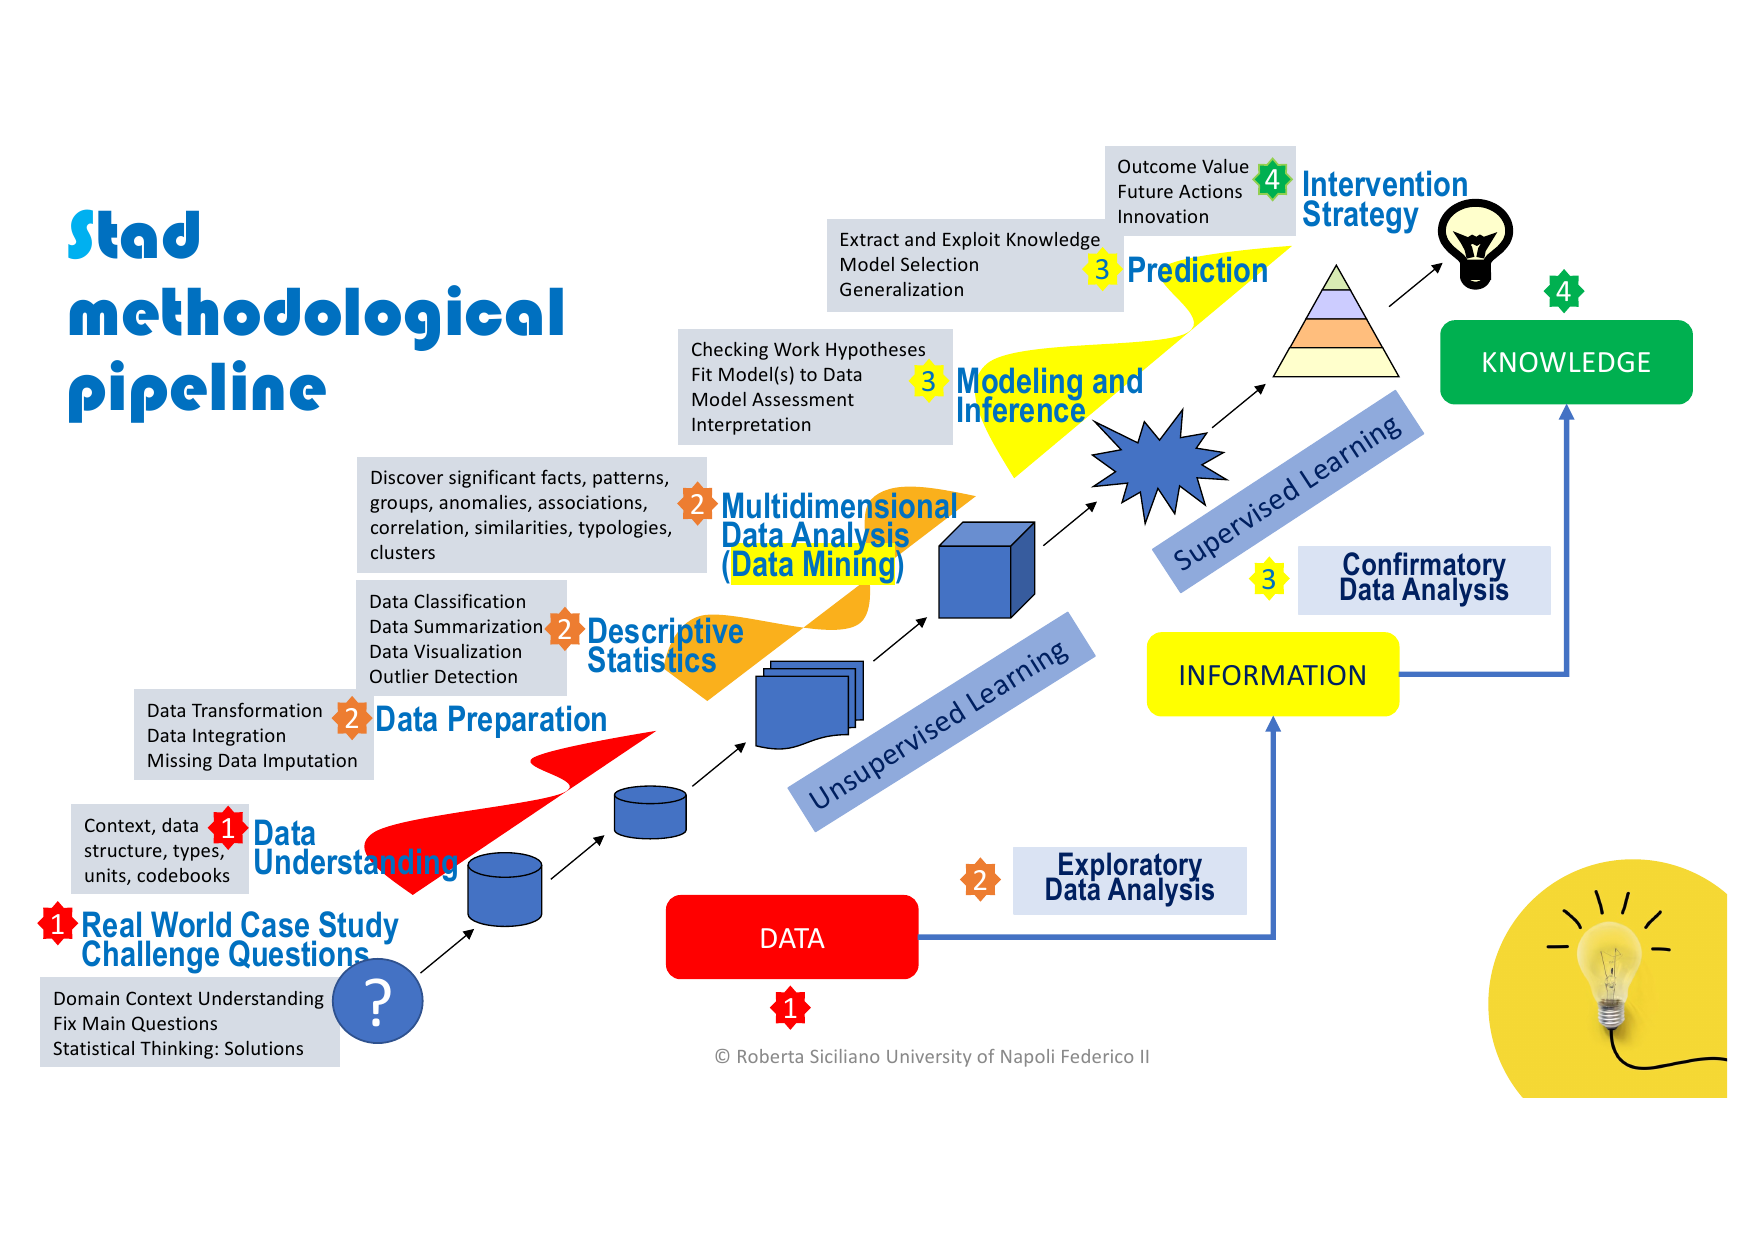
\includegraphics[width=0.85\textwidth]{slide_009}
    \caption{The Stad methodological pipeline: from a real-world case study and raw data, through data preparation, descriptive statistics and multidimensional data analysis (unsupervised learning), to modeling, inference and prediction (supervised learning), up to knowledge and intervention strategy.}
    \captionsetup{font=footnotesize}
\end{figure}

Reading the diagram left to right:
\begin{itemize}
  \item \texttt{Step 1 --- Real-world case study}: understand the domain, fix the main questions, think statistically about candidate solutions; this yields \textbf{data} together with an understanding of its context, structure, types, and codebooks.
  \item \texttt{Step 2 --- Data preparation \& exploratory analysis}: transform, integrate, and impute missing data; then describe it (classification, summarization, visualization, outlier detection) and mine it for patterns via \textbf{unsupervised learning}. This turns data into \textbf{information}.
  \item \texttt{Step 3 --- Modeling and inference}: fit model(s) to the data, assess and interpret them via \textbf{supervised learning}, checking work hypotheses through \textbf{confirmatory data analysis}. This turns information into \textbf{knowledge}.
  \item \texttt{Step 4 --- Intervention strategy}: use the knowledge to extract and exploit outcome value, decide future actions, and drive innovation.
\end{itemize}

\begin{noteboxtitle}{The big picture}
This pipeline is the skeleton of the entire course: unsupervised learning (Module A topics such as clustering) sits in the middle steps, supervised learning and reinforcement learning sit in the modeling/inference step, and everything is ultimately in service of turning data into a decision.
\end{noteboxtitle}

\subsection{Course structure: Module A vs Module B, educational aims}\label{sec:prolusion-structure}

\subsubsection{Two modules, one course}

\textbf{Advanced Statistical Learning and Modeling} is worth 12 CFU overall (first semester) and splits into two 6-CFU modules:

\begin{itemize}
  \item \textbf{Module A --- Advanced Statistical Learning} (Prof. Roberta Siciliano): probabilistic machine learning, \textbf{including reinforcement learning} --- this is the module this set of notes belongs to.
  \item \textbf{Module B --- Advanced Statistical Models} (Prof. Giulia Vannucci): generalized linear models, fixed and random effects, multi-level models, and Global Sensitivity Analysis.
\end{itemize}

\subsubsection{Educational aims}

The course as a whole aims to give students advanced statistical methodologies spanning both the classical and the modern (machine-learning) paradigm:
\begin{itemize}
  \item \textbf{Module A} provides modern statistical learning methodologies centered on probabilistic machine learning, including reinforcement learning.
  \item \textbf{Module B} provides generalized linear models and multi-level models (fixed and random effects), plus the methodological insights of Global Sensitivity Analysis to manage uncertainty in statistical models and probabilistic machine learning.
\end{itemize}

\begin{noteboxtitle}{Where reinforcement learning fits}
Reinforcement learning is explicitly named as part of Module A's probabilistic machine learning content: the rest of these notes (from the next chunk onward) build up the probabilistic view of ML, supervised learning foundations, and then reinforcement learning itself, following exactly this course map.
\end{noteboxtitle}

\subsection{What is Machine Learning?}\label{sec:rl-intro-what-is-ml}

\subsubsection{A working definition}

A classic and still very useful definition of Machine Learning comes from Tom Mitchell:

\begin{defbox}{Machine Learning (Mitchell, 1997)}
``A computer program is said to learn from \textbf{experience $E$} with respect to some class of \textbf{tasks $T$}, and \textbf{performance measure $P$}, if its performance at tasks in $T$, as measured by $P$, improves with experience $E$.''

\textit{In other words: a system ``learns'' if, after seeing more data (experience), it gets better at some job (task), and we have a way to check that it is actually getting better (performance measure).}
\end{defbox}

The right ML tool to use for a problem depends on three things:
\begin{itemize}
  \item the nature of the \textbf{task} $T$ we want the system to learn (e.g.\ classify emails, predict a price, choose an action);
  \item the nature of the \textbf{performance measure} $P$ we use to judge success (e.g.\ accuracy, mean squared error, cumulative reward);
  \item the nature of the \textbf{experience} $E$ we give it (e.g.\ labeled examples, raw unlabeled data, trial-and-error interaction).
\end{itemize}

When the goal is \textbf{prediction} -- guessing something we do not yet know -- it becomes natural, and very useful, to think about ML through the lens of probability.

\subsubsection{The probabilistic perspective}

\begin{defbox}{Probabilistic view of ML}
Probability is the mathematical formalization of \textit{uncertainty}. Any unknown quantity -- a future value, a missing label, the parameters of a model -- is treated as a \textbf{random variable} that follows a \textbf{probability distribution}, i.e.\ a weighted list of the values it could take and how likely each one is.

\textit{Think of it this way: instead of saying ``the price tomorrow will be \$105'', we say ``the price tomorrow is a random variable, and \$105 is the most likely value, but \$100 or \$110 are also plausible''.}
\end{defbox}

Why bother with this probabilistic framing? Two main reasons are usually given:

\begin{itemize}
  \item it is the \textit{optimal approach to decision making under uncertainty} -- if you must act without knowing the true outcome, weighting options by their probability is the principled way to do it;
  \item probabilistic modeling is the \textit{common language} of many other fields (stochastic optimization, control theory, econometrics, information theory, statistical physics, bio-statistics), so it provides a \textbf{unifying framework} across disciplines.
\end{itemize}

As E.\,T.\ Jaynes put it, the rules of probability are not just for counting frequencies of random events -- they are the unique rules for conducting \textit{any} kind of plausible reasoning. Almost the whole of modern ML can be recast in these probabilistic terms, which is why this perspective is worth having in mind from day one.

\subsubsection{The three types of Machine Learning}

There are three broad families of ML problems, distinguished by \textit{what kind of experience} the system is given:

\begin{itemize}
  \item \textbf{Unsupervised (exploratory) learning}: only inputs, no target -- the goal is to find structure in the data itself;
  \item \textbf{Supervised (predictive) learning}: inputs paired with a known target/output -- the goal is to predict the target for new inputs (see Section~\ref{sec:rl-intro-supervised});
  \item \textbf{Reinforcement learning}: an agent interacts with an environment and learns from rewards/punishments received along the way (see Section~\ref{sec:rl-intro-rl}).
\end{itemize}

\begin{figure}[H]
    \centering
    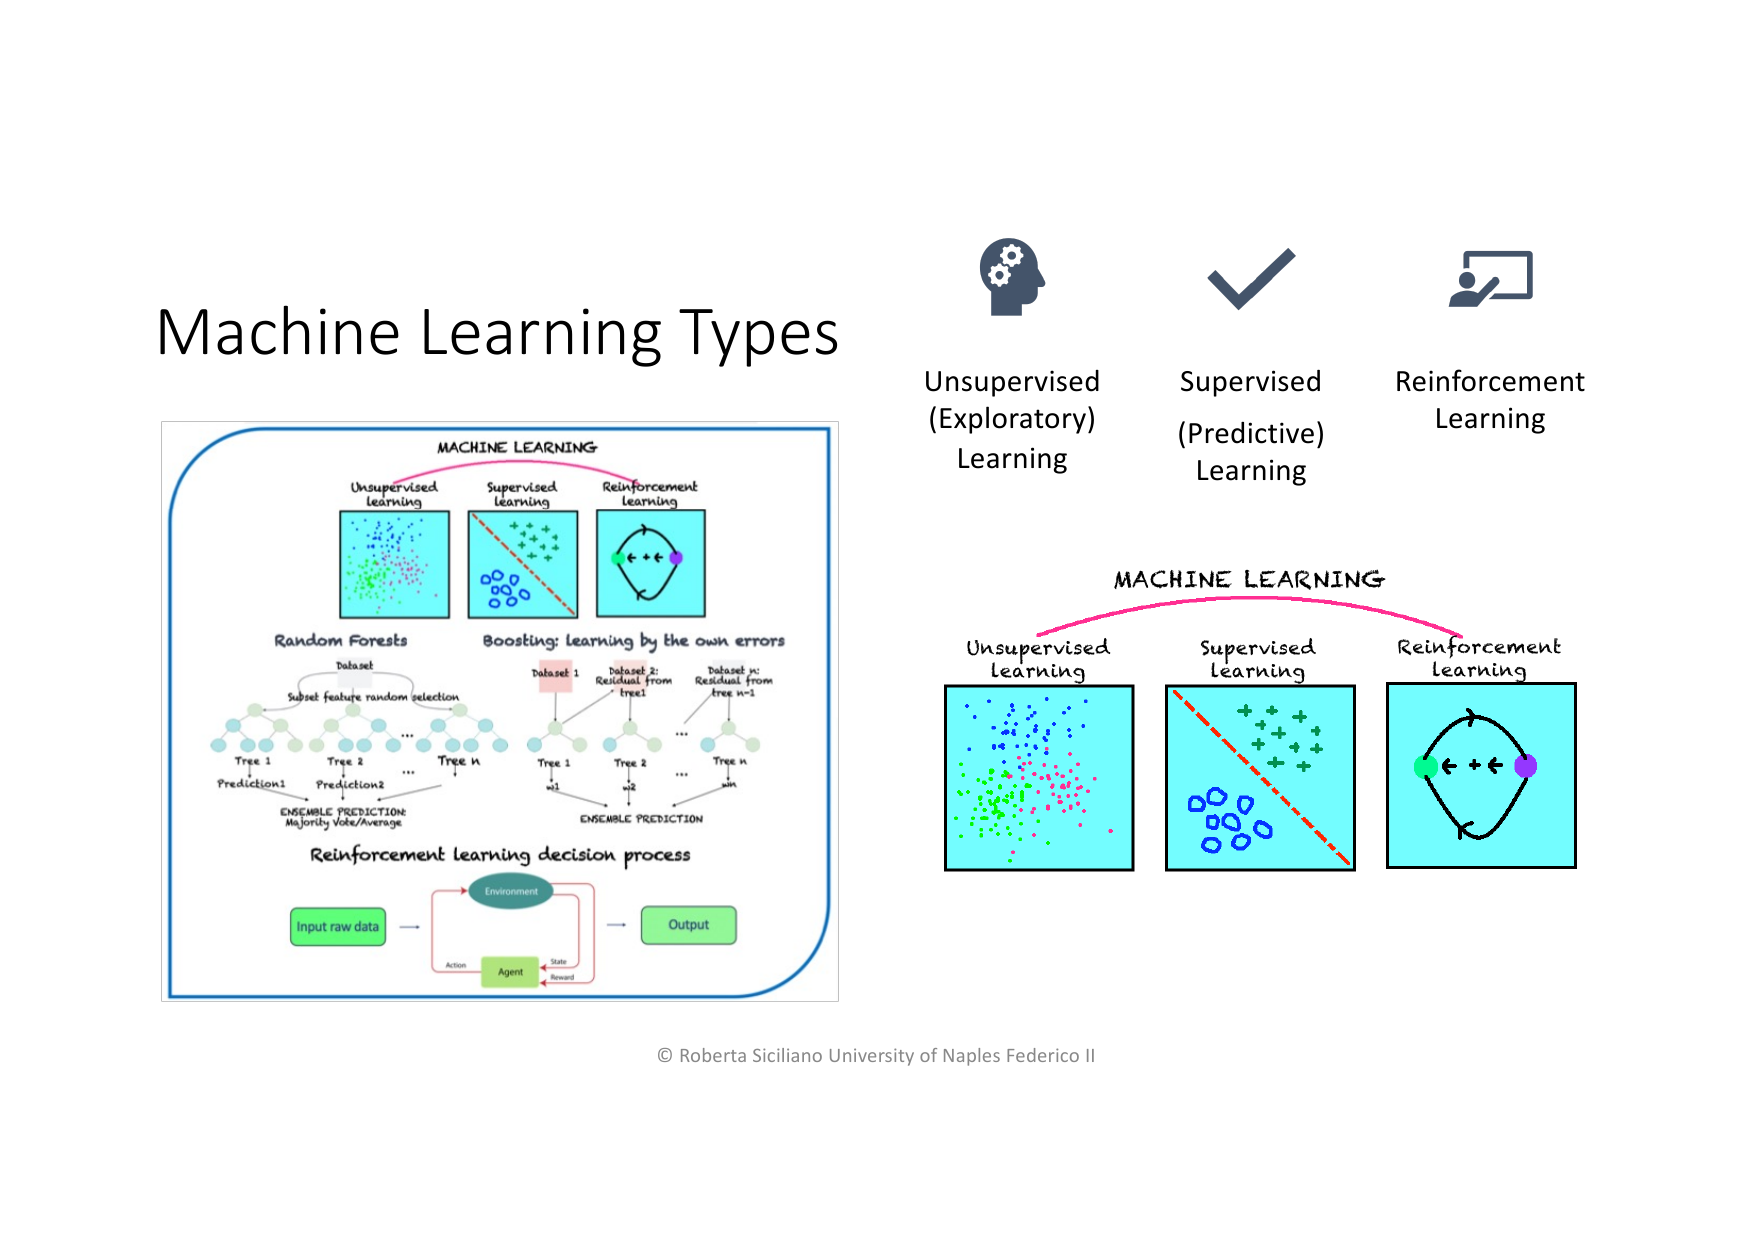
\includegraphics[width=0.85\textwidth]{slide_016}
    \caption{The three Machine Learning types and a few representative algorithms/pipelines for each.}
    \captionsetup{font=footnotesize}
\end{figure}

A short, intuitive summary of the three tools:

\begin{itemize}
  \item \textbf{Unsupervised learning}: all features play the same role -- they are all just ``inputs'', and there is no target to predict.
  \item \textbf{Supervised learning}: uses statistical/ML models to predict or estimate an output based on one or more inputs.
  \item \textbf{Reinforcement learning}: simplifies the learning of complex behaviors via reward-driven trial and error -- learning \textit{how to act} when only occasional reward or punishment signals are available. (A natural analogy: this is roughly how a baby learns to walk -- no one hands it labeled examples of ``correct'' steps, it just tries, falls, and adjusts.)
\end{itemize}

\subsection{Unsupervised Learning}\label{sec:rl-intro-unsupervised}

\subsubsection{Goal and setup}

\begin{defbox}{Unsupervised learning}
The goal is ``to make sense of data'': finding interesting patterns without any labeled target. All variables play the same role in the analysis,
\[
  \mathcal{D} = \{\mathbf{x}_n\}_{n=1}^{N},
\]
and we typically fit an \textbf{unconditional} model $p(\mathbf{x})$ that can, in principle, generate new data points similar to the ones observed.

\textit{Here $\mathcal{D}$ is just the dataset ($N$ observations $\mathbf{x}_n$, no labels attached), and $p(\mathbf{x})$ is a probability distribution over the data itself -- learning it means learning ``what typical data looks like''.}
\end{defbox}

\subsubsection{The main unsupervised tasks}

\begin{itemize}
  \item \textbf{Clustering}: discover groups of similar examples within the data.
  \item \textbf{Density estimation}: determine how the data is distributed across the feature space.
  \item \textbf{Dimensionality reduction}: project the data from a high-dimensional space onto a much smaller (2D or 3D) subspace, e.g.\ for visualization (this is exactly what PCA does, see Section~\ref{sec:rl-intro-pca}).
  \item \textbf{Graphical models}: discover which variables are correlated with which, using graph theory to represent dependencies.
  \item \textbf{Frequent itemset mining / association rules}: discover subsets of items that tend to be bought together (classic ``market basket'' analysis).
\end{itemize}

\subsubsection{How do we measure performance without labels?}

This is the tricky part: in unsupervised learning there is \textbf{no ground truth} to compare against, unlike in supervised learning where we can just check predictions against known labels.

A common workaround is to measure the probability the model assigns to \textit{unseen} test examples, via the (unconditional) negative log-likelihood of the data:
\[
  \mathcal{L}(\boldsymbol{\theta}; \mathcal{D}) = -\frac{1}{|\mathcal{D}|} \sum_{\mathbf{x} \in \mathcal{D}} \log p(\mathbf{x} \mid \boldsymbol{\theta}).
\]
Here $\boldsymbol{\theta}$ are the model's parameters, $|\mathcal{D}|$ is the number of data points, and $p(\mathbf{x}\mid\boldsymbol{\theta})$ is the probability the model assigns to a given data point.

\textit{Intuition: a good model is not ``surprised'' by real data -- it assigns high probability to regions where data actually occurs, and low probability elsewhere. A low (negative log-likelihood) score means the model has learned the typical patterns in the data, similarly to what happens in density estimation.}

Unfortunately, density estimation is genuinely hard in high dimensions. A popular alternative evaluation strategy is to use the learned unsupervised representation as \textbf{features for a downstream supervised task}: if the unsupervised method really discovered useful structure, a supervised model built on top of it should need much less labeled data to perform well than one built on the raw features.

\subsection{Principal Component Analysis}\label{sec:rl-intro-pca}

\subsubsection{Discovering latent factors}

Principal Component Analysis (PCA) is the workhorse technique for dimensionality reduction: it looks for a small number of \textbf{latent factors} that explain most of the variability in high-dimensional data.

\textit{Example: when modeling the appearance of face images, there might be only a handful of underlying factors -- lighting, pose, identity -- that account for most of the differences between pictures, even though each image itself has thousands of pixels.}

\subsubsection{Where PCA (and its variants) show up}

\begin{itemize}
  \item \textbf{Biology}: PCA is routinely used to interpret gene microarray data, since each measurement is really the joint outcome of many genes that are correlated because they belong to shared biological pathways (see the genetics example in Section~\ref{sec:rl-intro-genetics}).
  \item \textbf{Natural Language Processing}: a PCA variant called \textbf{Latent Semantic Analysis} is used for document retrieval.
  \item \textbf{Signal processing} (e.g.\ acoustic or neural signals): \textbf{Independent Component Analysis} (another PCA variant) separates a mixture of signals into its different sources -- for instance, EEG brain scans record neuronal activity indirectly through electromagnetic signals picked up at sensors on the head, and ICA helps disentangle the underlying sources.
  \item \textbf{Non-Negative Matrix Factorization}: a variant of PCA where both data and components are constrained to be non-negative, which is natural for data like images (pixel intensities cannot be negative).
  \item \textbf{Computer graphics}: motion-capture data is often projected to a low-dimensional space to help create animations.
\end{itemize}

\subsection{Genetics Examples}\label{sec:rl-intro-genetics}

\subsubsection{DNA microarrays}

A classic application area for unsupervised learning is the analysis of \textbf{DNA microarrays} of gene expression: each cell in the data matrix records how strongly a gene is expressed in a given sample.

\begin{figure}[H]
    \centering
    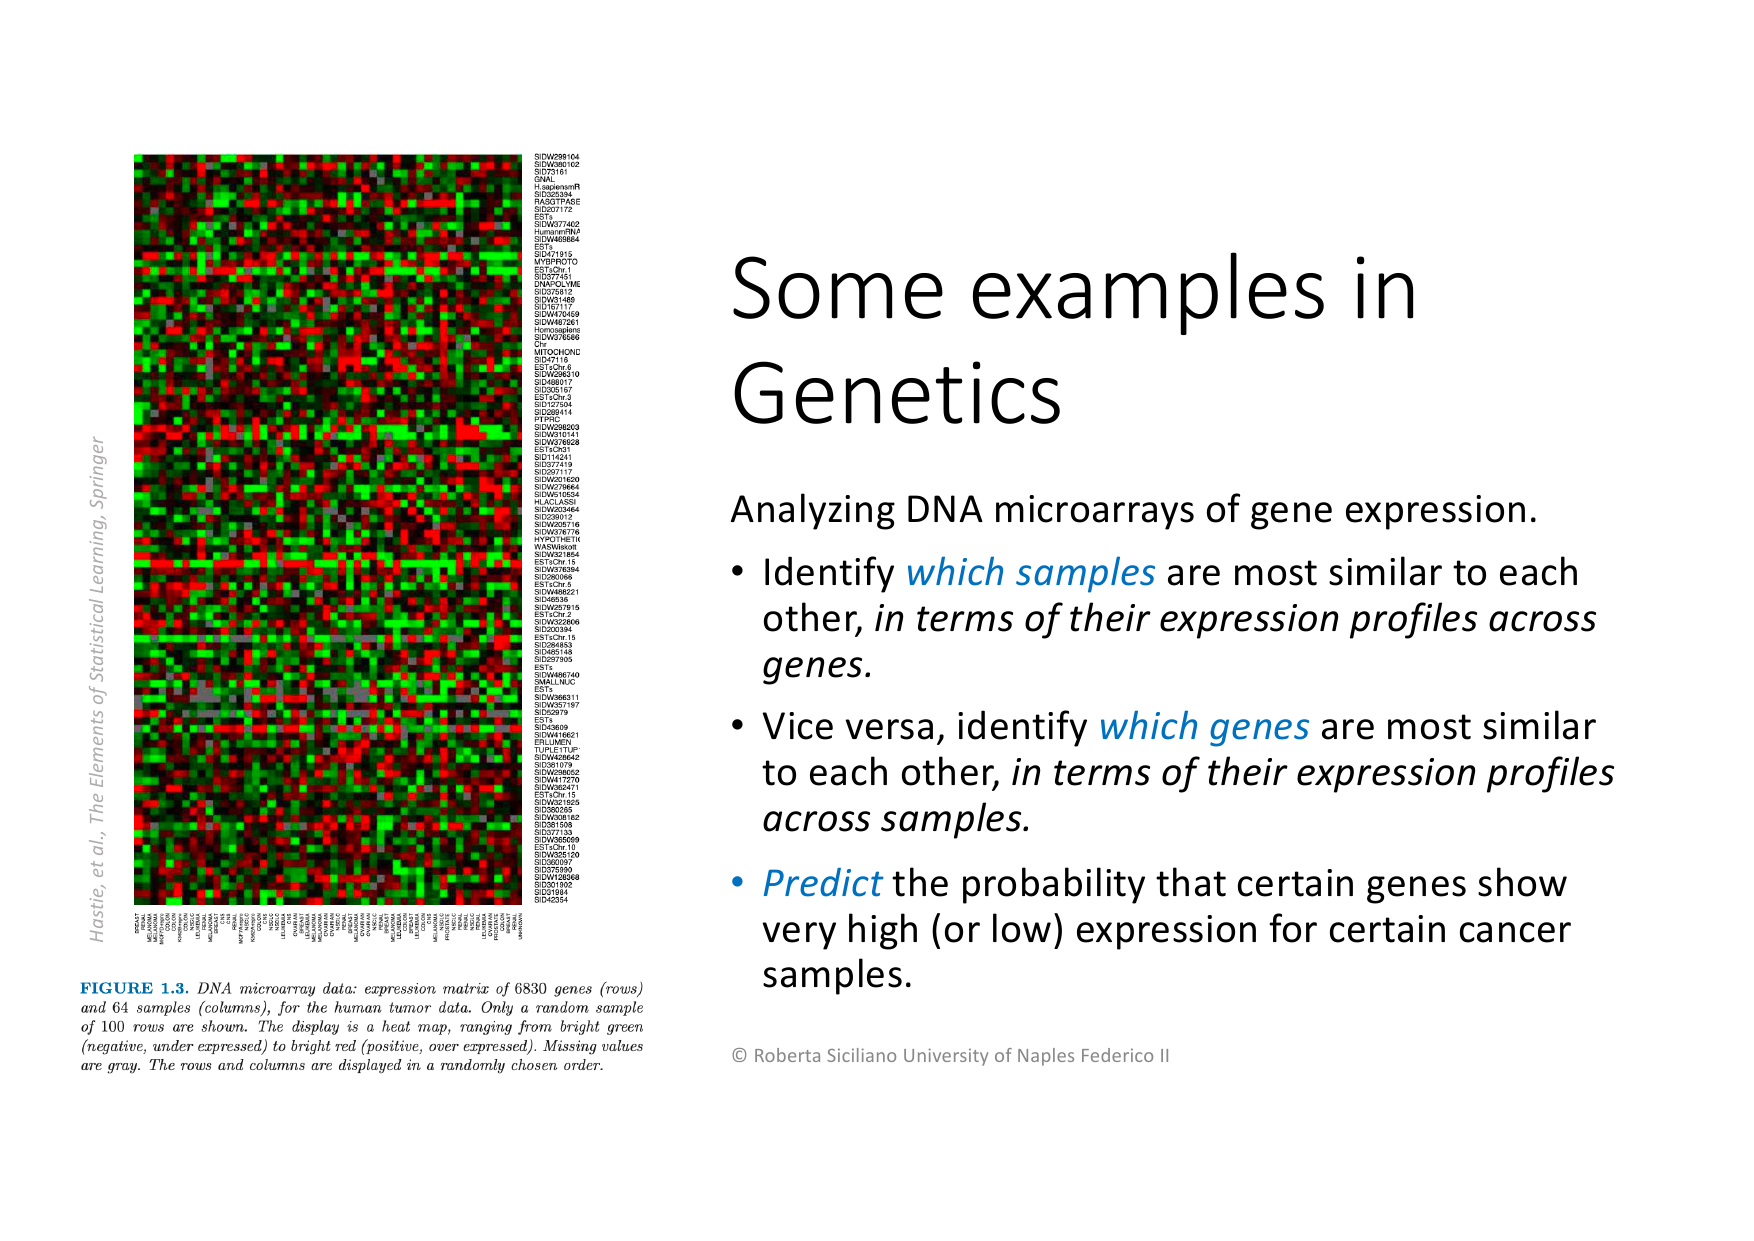
\includegraphics[width=0.60\textwidth]{slide_021}
    \caption{DNA microarray data: expression matrix of 6{,}830 genes (rows) by 64 samples (columns), shown as a heat map (bright green = under-expressed, bright red = over-expressed). Source: Hastie et al., \textit{The Elements of Statistical Learning}.}
    \captionsetup{font=footnotesize}
\end{figure}

With this kind of data, unsupervised learning can answer several natural questions:
\begin{itemize}
  \item identify \textbf{which samples} are most similar to each other, in terms of their expression profiles across genes;
  \item vice versa, identify \textbf{which genes} are most similar to each other, in terms of their expression profiles across samples;
  \item \textbf{predict} the probability that certain genes show very high (or low) expression in certain cancer samples.
\end{itemize}

\subsubsection{Gene expression as a clustering problem}

A concrete illustration uses the \textbf{NCI60} dataset: 6{,}830 gene expression measurements for each of 64 cancer cell lines, spanning 14 different cancer types. Since there are thousands of gene measurements per cell line, direct visualization is essentially impossible -- this is exactly the setting where dimensionality reduction (PCA) becomes essential, projecting the data down to two components $Z_1, Z_2$ that can actually be plotted.

\begin{figure}[H]
    \centering
    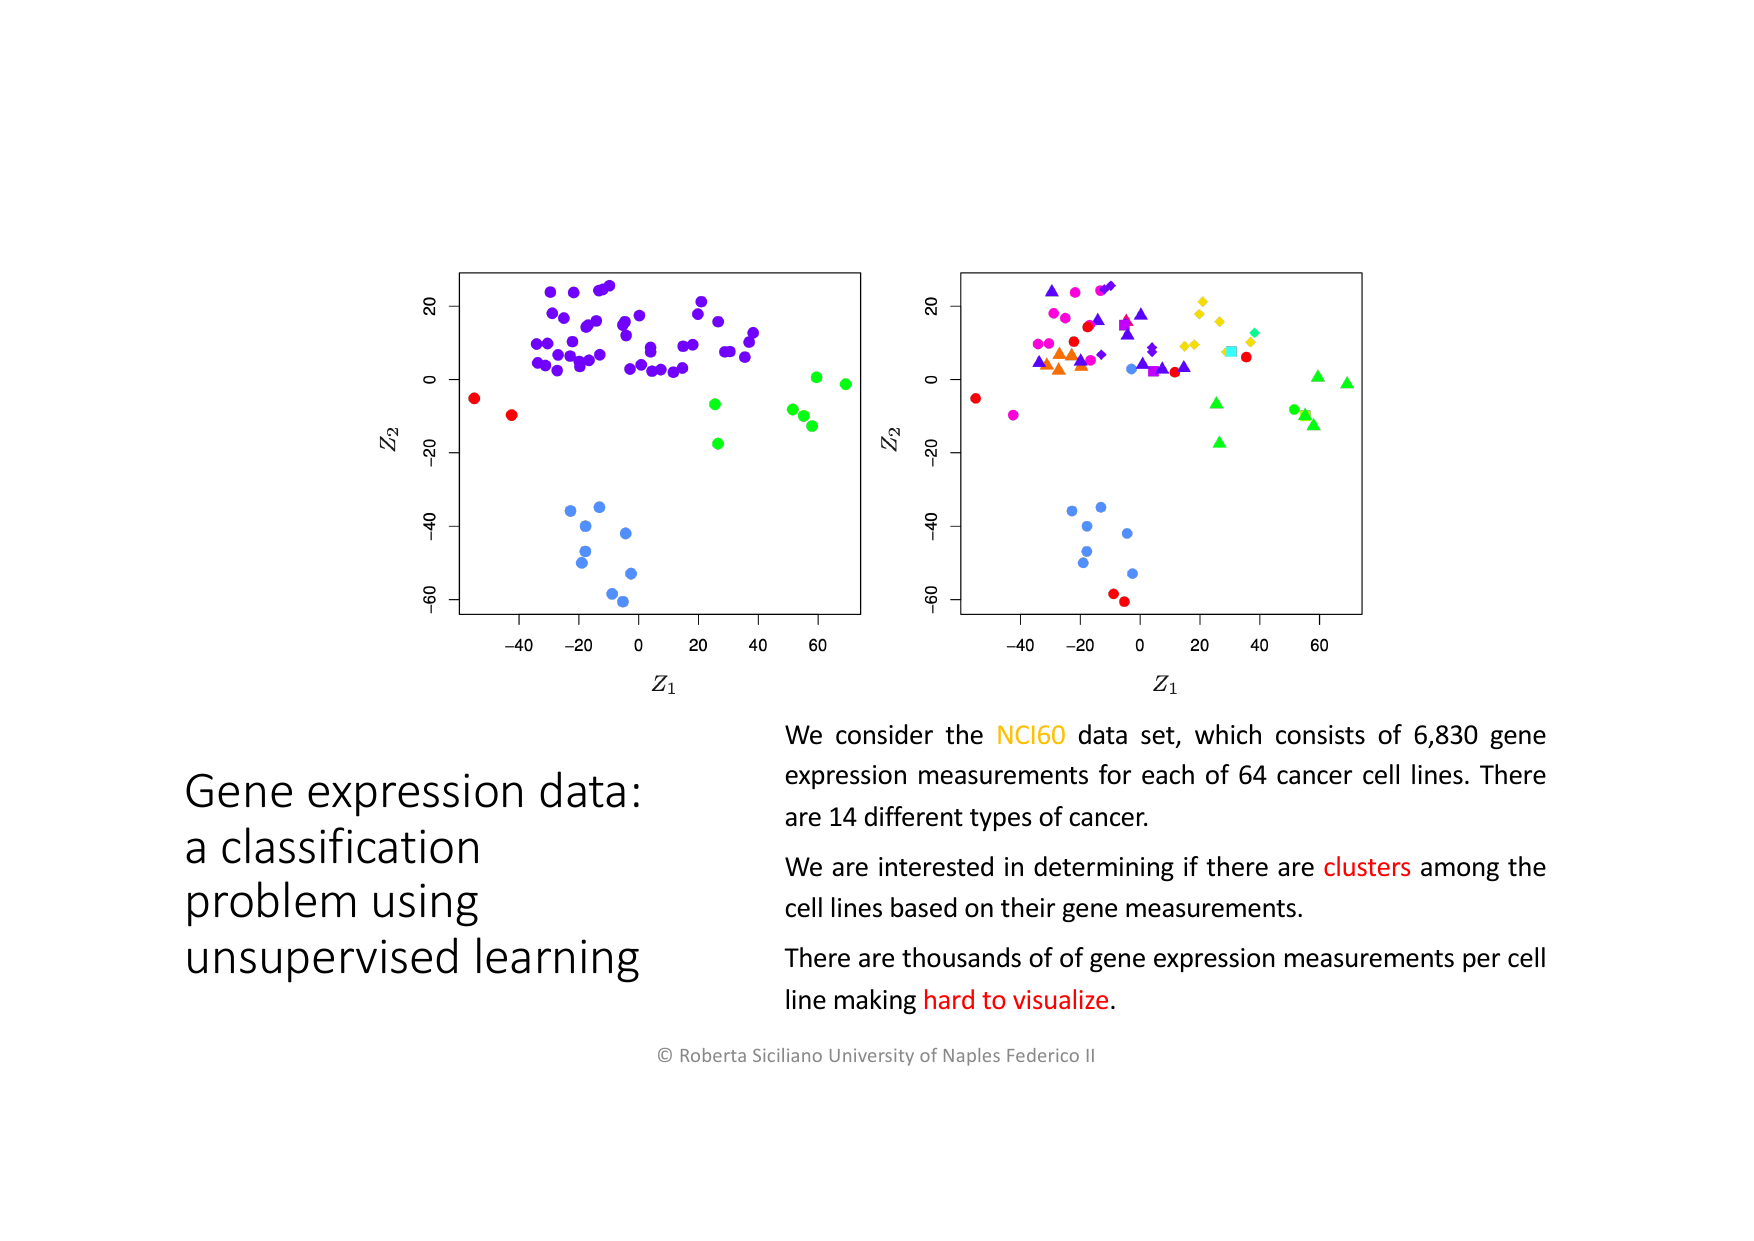
\includegraphics[width=0.85\textwidth]{slide_022}
    \caption{Gene expression data (NCI60) projected onto its first two principal components. Left: colored by discovered cluster; right: colored by true cancer type. Clusters found in an unsupervised way largely align with the real cancer types.}
    \captionsetup{font=footnotesize}
\end{figure}

The question being asked is: do cell lines with similar gene expression profiles also correspond to the same type of cancer? Comparing the unsupervised clusters (left panel) against the known cancer types (right panel) shows a strong -- though not perfect -- agreement, which is encouraging evidence that the discovered structure is biologically meaningful.

\subsection{Matrix Completion}\label{sec:rl-intro-matrix-completion}

\subsubsection{Filling in the blanks}

\begin{defbox}{Matrix completion}
The goal of \textbf{imputation} is to infer plausible values for missing entries in a data matrix, typically marked as \texttt{NaN} (``Not a Number'').

\textit{Think of a big spreadsheet with holes in it: matrix completion tries to guess sensible values for those holes using the patterns present in the entries we do observe.}
\end{defbox}

Two classic applications:

\begin{itemize}
  \item \textbf{Image inpainting}: ``fill in'' holes in an image (e.g.\ due to scratches or occlusions) with realistic texture, effectively denoising the image by imputing the hidden pixels. This can be tackled by building a joint probability model of the pixels from a set of clean images, and then inferring the unknown pixels given the known ones.
  \item \textbf{Collaborative filtering}: the typical example is predicting which movies people will want to watch, based on how they -- and other people -- have rated movies they have already seen. The key idea is that the prediction relies mainly on the \textbf{ratings matrix} itself (users $\times$ movies), not necessarily on explicit features of the movie or the user.
\end{itemize}

\subsection{Self-Supervised and Semi-Supervised Learning}\label{sec:rl-intro-self-semi-supervised}

\subsubsection{Self-supervised learning}

\begin{defbox}{Self-supervised learning}
We create a \textbf{proxy supervised task} directly from unlabeled data: the model trains itself to predict one part of the input from another part of the same input.

\textit{Example: predict a color image from its grayscale version, or mask out some words in a sentence and try to predict them from the surrounding context (this is essentially how modern language models are pre-trained).}
\end{defbox}

Formally, the resulting predictor is
\[
  \hat{x}_1 = f(x_2; \theta),
\]
where $x_2$ is the observed part of the input and $x_1$ is the part being predicted, with $\theta$ the model parameters.

\textit{The hope is that, in order to get good at this proxy task, the model is forced to learn genuinely useful features -- features that can then be reused for standard downstream supervised tasks, even when very little labeled data is available for those.}

\subsubsection{Semi-supervised learning}

\begin{defbox}{Semi-supervised learning}
We use \textbf{both labeled and unlabeled data} together to improve a supervised model.
\end{defbox}

A typical recipe: train the model on the labeled images as usual; then, for each unlabeled image, apply two different data augmentations to create two ``views'' of it, and add a training signal that pushes the model to predict the \textit{same} label for both augmented views (e.g.\ via a cross-entropy term added to the loss).

\textit{Intuition: if two augmented versions of the same underlying image are really ``the same thing'', a good model should agree with itself on both -- this lets unlabeled data still contribute useful training signal, even without a true label attached.}

\subsection{Supervised Learning: Setup and the Two Cultures}\label{sec:rl-prolusion-supervised-setup}

In supervised learning the variables are not all equal: some play the role of ``causes'' and some the role of ``effects''. The task $T$ is to learn a mapping $f$ from inputs $\mathbf{x} \in \mathcal{X}$ to outputs $\mathbf{y} \in \mathcal{Y}$.

\begin{itemize}
  \item The \textbf{inputs} $\mathbf{x}$ are the explanatory (or exogeneous) variables, also called covariates or \textit{predictors}. They are fixed-dimensional vectors, $\mathcal{X} = \mathbb{R}^D$.
  \item The \textbf{outputs} $\mathbf{y}$ are the \textit{targets}, responses, or endogeneous variables.
  \item The \textbf{experience} $E$ is a set of $N$ input-output pairs, known as the \textbf{training set} (or learning set):
  \[
    \mathcal{D} = \{(\mathbf{x}_n, \mathbf{y}_n)\}_{n=1}^{N}.
  \]
  Here $N$ is simply the sample size, i.e.\ how many labelled examples we have to learn from.
  \item The \textbf{performance measure} $P$ depends on what kind of output we are predicting (a number, a category, a probability distribution\dots).
\end{itemize}

\textit{Intuition:} think of $\mathcal{D}$ as a table of exercises with the solutions already filled in ($\mathbf{x}_n$ = the exercise, $\mathbf{y}_n$ = the solution). The learning machine studies this table so that, later, it can solve new exercises it has never seen.

Two complementary reasons to build a model:
\begin{itemize}
  \item \textbf{Prediction}: being able to guess $\mathbf{y}$ for future values of $\mathbf{x}$.
  \item \textbf{Information}: understanding \emph{how} nature links $\mathbf{x}$ to $\mathbf{y}$.
\end{itemize}

\subsubsection{Breiman's Two Cultures}

Leo Breiman's famous 2001 paper \textit{``Statistical Modeling: the Two Cultures''} contrasts two very different philosophies for doing statistical modeling.

\begin{defbox}{Data Modeling Culture}
Assume the data were generated by a known stochastic model (e.g.\ linear regression, logistic regression, Cox model), fit its parameters, and use the fitted model both for prediction and for interpretation.
\begin{itemize}
  \item Model validation relies on goodness-of-fit tests and residual analysis.
  \item Conclusions are about \emph{the model's} mechanism, not necessarily about nature's real mechanism: if the model is a poor emulation of reality, the conclusions can be wrong.
  \item Prediction is rarely perfect: unmeasured variables contribute what is called ``noise''. How well the model box reproduces nature's box measures how good the model really is.
\end{itemize}
\textit{Think of it as: pick an equation you believe in, then check if it fits.}
\end{defbox}

\begin{defbox}{Algorithmic Modeling Culture}
Treat the true input-output mechanism as unknown, and instead search for a function or algorithm (decision trees, neural nets, \dots) that predicts well, without committing to an explicit statistical model.
\begin{itemize}
  \item Model validation relies on prediction accuracy measures (how many mistakes does it make?), not on distributional assumptions.
  \item Vapnik's Statistical Learning Theory provides bounds on the generalization error (the error on unseen data) that depend on the ``capacity'' — roughly, the flexibility — of the algorithm.
\end{itemize}
\textit{Think of it as: don't guess the equation, just let a flexible algorithm find the pattern, and measure how well it predicts.}
\end{defbox}

\begin{figure}[H]
    \centering
    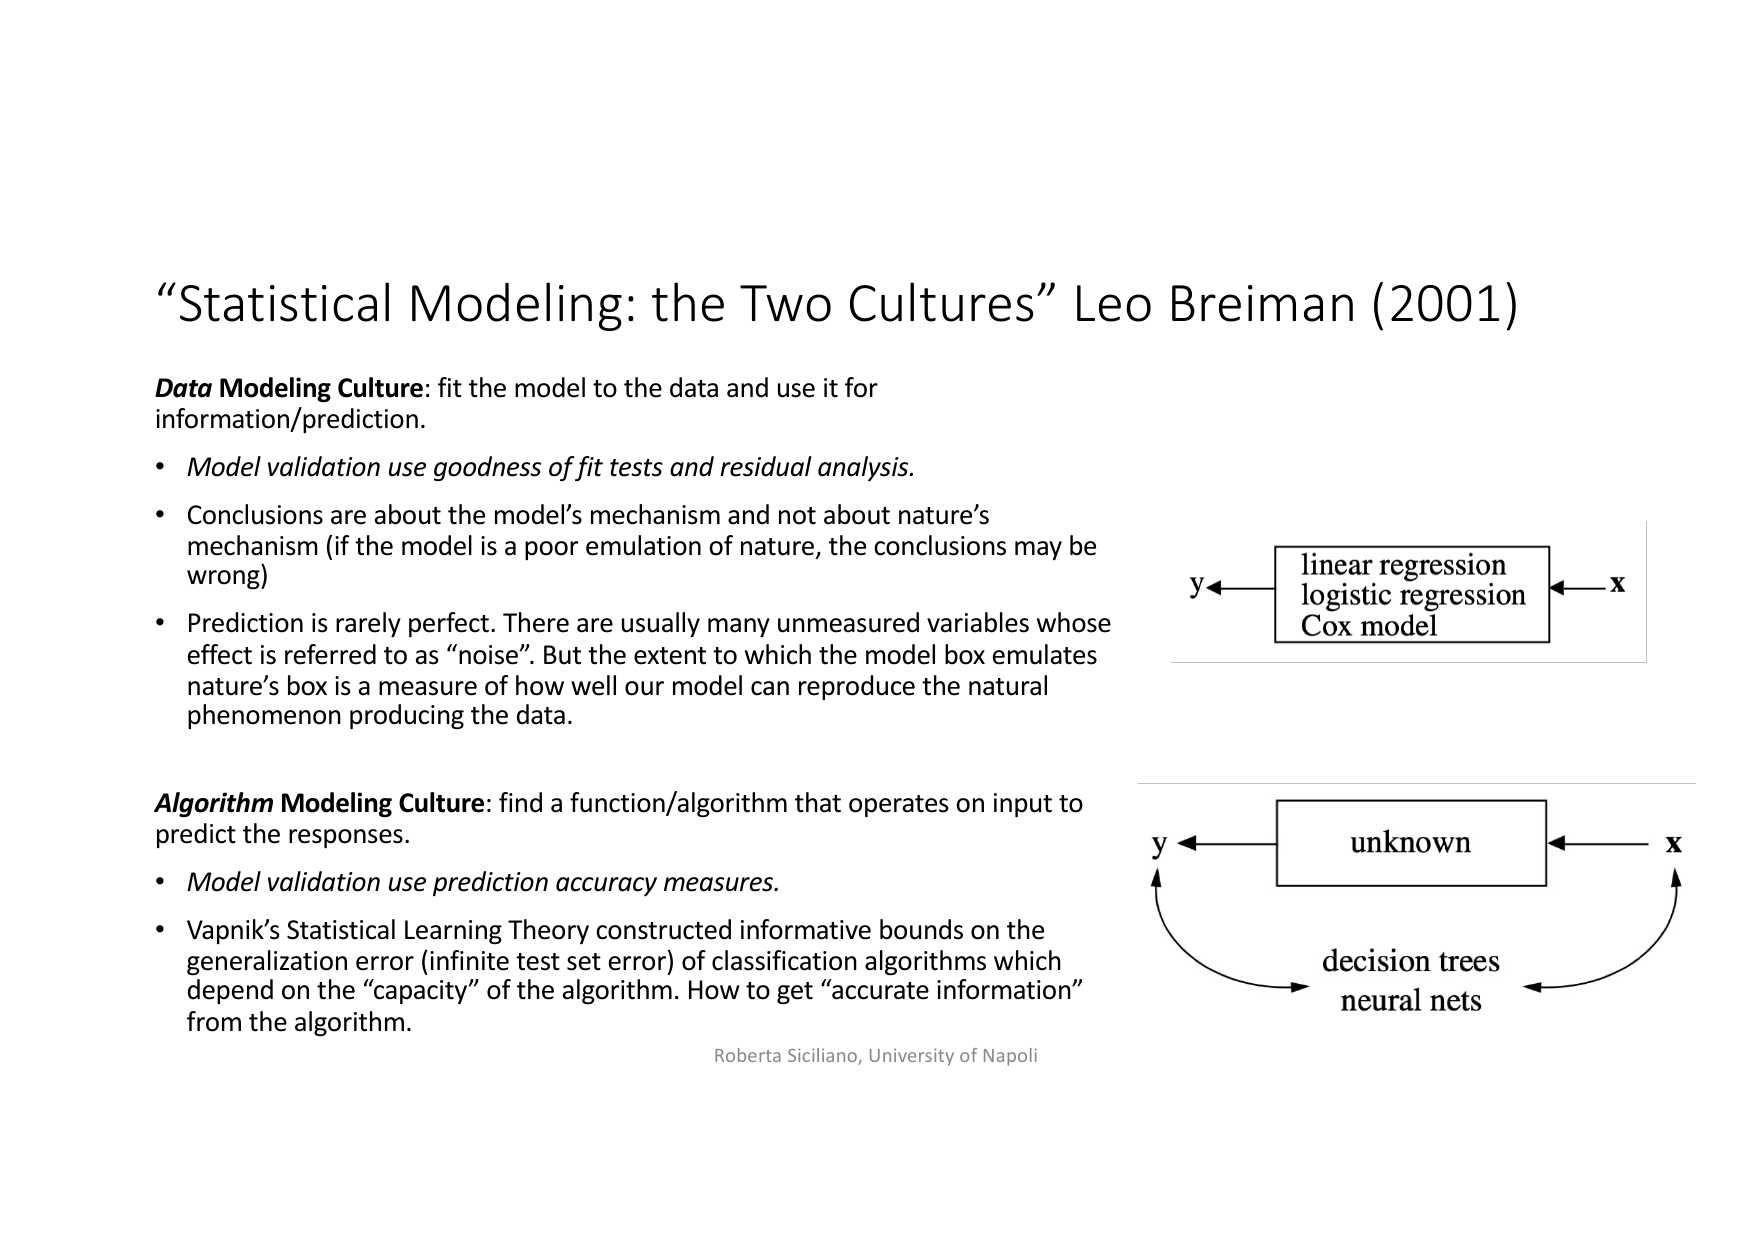
\includegraphics[width=0.85\textwidth]{slide_026}
    \caption{Data modeling culture (a known model connects $\mathbf{x}$ to $\mathbf{y}$) versus algorithmic modeling culture (an unknown function, approximated by flexible algorithms such as decision trees or neural nets).}
    \captionsetup{font=footnotesize}
\end{figure}

The three keywords on the opening slide summarize the tensions running through the whole course:
\begin{itemize}
  \item \textbf{Rashomon}: many different models can fit the data almost equally well (multiplicity of good models) — which one do we trust?
  \item \textbf{Occam}: the trade-off between a simple model and an accurate one.
  \item \textbf{Bellman}: is having many dimensions/variables a curse (too much complexity) or a blessing (more information)?
\end{itemize}

\subsection{The Generator-Supervisor-Learning Machine Framework}\label{sec:rl-prolusion-gslm}

\subsubsection{The three components}

Vapnik's classical framework describes learning as an interaction between three abstract components.

\begin{defbox}{Generator, Supervisor, Learning Machine}
\begin{itemize}
  \item A \textbf{Generator} $G$ produces random input vectors $\mathbf{x} \in \mathbb{R}^D$, drawn independently from a fixed but unknown probability distribution $p(\mathbf{x})$.
  \item A \textbf{Supervisor} $S$ returns an output $y$ for every input $\mathbf{x}$, according to a conditional distribution $p(y \mid \mathbf{x})$, also fixed but unknown.
  \item A \textbf{Learning Machine} $LM$ observes the training sample (pairs of $\mathbf{x}$ and the supervisor's answer $y$, drawn according to the joint distribution $p(\mathbf{x}, y) = p(\mathbf{x}) p(y \mid \mathbf{x})$) and is capable of implementing a family of functions $f(\mathbf{x}, \boldsymbol\theta)$, indexed by parameters $\boldsymbol\theta \in \boldsymbol\Theta$.
\end{itemize}
\textit{Think of it as: nature generates questions (G), nature also knows the true answers (S), and the machine (LM) tries to guess the answers, learning from examples of question-answer pairs.}
\end{defbox}

During training, the LM builds an operator (a predictor) that produces a guess $\hat{y}$ for any input $\mathbf{x}$ generated by $G$. The two goals of learning are:
\begin{itemize}
  \item \textbf{Generalize}: learn from the training sample so as to give useful answers (predictions, decisions) on \emph{new}, unseen cases.
  \item \textbf{Find the best functional relationship}: identify, within the family $f(\mathbf{x}, \boldsymbol\theta)$, the one that best approximates the supervisor's response, minimizing the discrepancy (this is sometimes called \textit{transductive inference}).
\end{itemize}

Model selection — deciding which $\boldsymbol\theta$, or which level of flexibility, is best — is typically done using a separate test sample or cross-validation.

\begin{figure}[H]
    \centering
    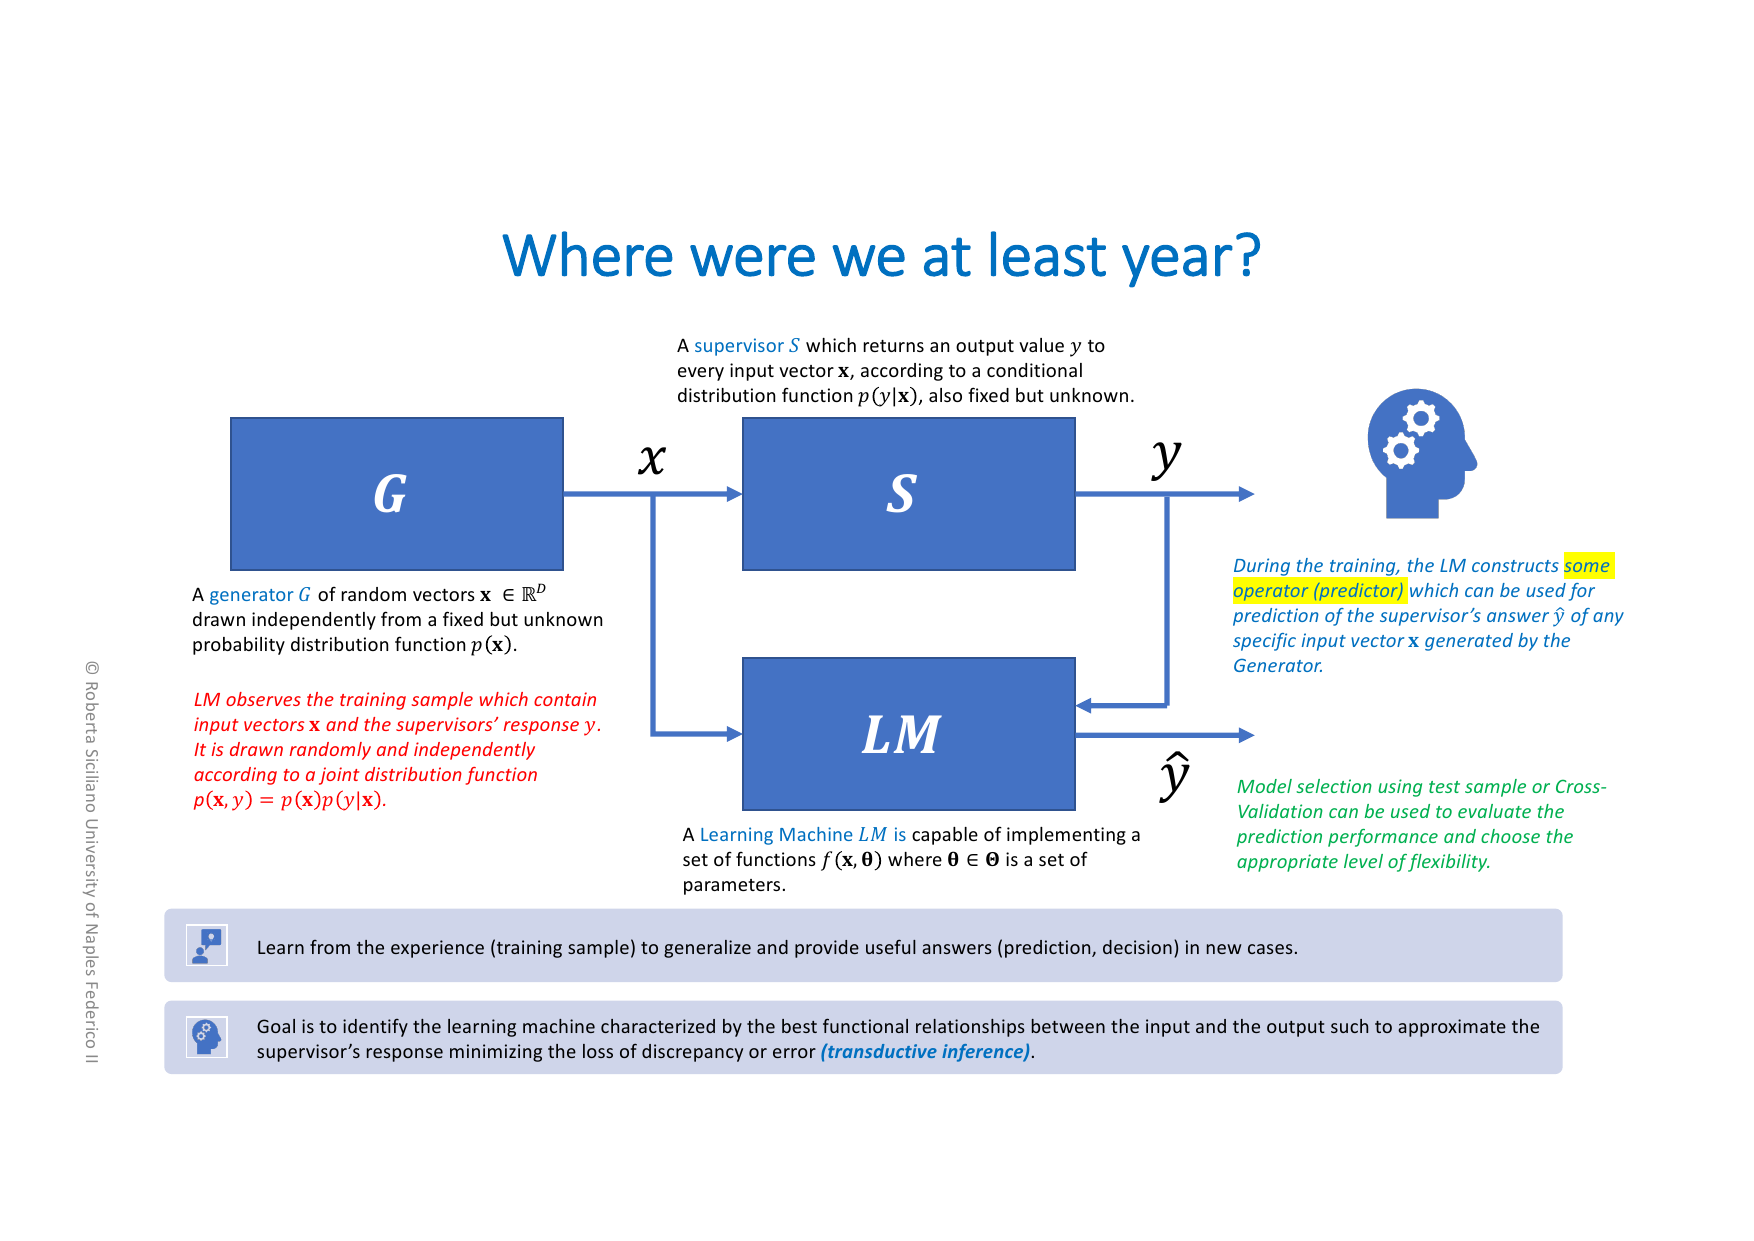
\includegraphics[width=0.85\textwidth]{slide_027}
    \caption{The Generator-Supervisor-Learning Machine (G-S-LM) framework.}
    \captionsetup{font=footnotesize}
\end{figure}

\subsubsection{Empirical Risk Minimization}

To choose the best $\boldsymbol\theta$ we need a way to \emph{measure} how wrong a prediction is, and then minimize that measure.

\begin{defbox}{Loss function}
The \textbf{loss function} $\ell\bigl(y, f(\mathbf{x}, \boldsymbol\theta)\bigr)$ measures the discrepancy between the true answer $y$ and the machine's prediction $f(\mathbf{x}, \boldsymbol\theta)$ for a single example.
\textit{Intuition: it is the ``penalty'' the machine pays for getting a specific example wrong — zero (or small) if the prediction is close to the truth, large otherwise.}
\end{defbox}

Given the loss, two related quantities matter:

\[
  R_{\text{emp}}(\boldsymbol\theta) = \mathcal{L}(\boldsymbol\theta) \triangleq \frac{1}{N}\sum_{n=1}^{N} \ell\bigl(y_n, f(\mathbf{x}_n, \boldsymbol\theta)\bigr)
\]
\begin{itemize}
  \item $R_{\text{emp}}(\boldsymbol\theta)$ (or $\mathcal{L}(\boldsymbol\theta)$) is the \textbf{empirical risk}: the average loss computed on the $N$ training examples we actually have.
  \item $N$: sample size; $n$: index running over the training examples.
\end{itemize}
\textit{Intuition: it is simply ``how many mistakes (or how big a mistake) did the model make, on average, on the data it was trained on''.}

\[
  R(\boldsymbol\theta) = \int \mathcal{L}\bigl(y, f(\mathbf{x}, \boldsymbol\theta)\bigr)\, dF(x, y)
\]
\begin{itemize}
  \item $R(\boldsymbol\theta)$ is the \textbf{risk functional} (also called expected risk or true risk): the average loss over \emph{all possible} data, according to the true (unknown) distribution $F(x,y)$.
\end{itemize}
\textit{Intuition: this is the error the model would make on brand-new, future data — the number we actually care about, but that we can never compute exactly because we don't know $F(x,y)$.}

\begin{defbox}{Empirical Risk Minimization (ERM)}
The \textbf{ERM criterion} chooses $\boldsymbol\theta$ by minimizing the empirical risk $R_{\text{emp}}(\boldsymbol\theta)$ over the training sample, as a stand-in for the (unobservable) true risk $R(\boldsymbol\theta)$.

ERM gives a \textbf{consistent estimate} if, as we feed it more and more functions $f(\mathbf{x}, \boldsymbol\theta)$, both the empirical risk and the expected risk converge to the smallest possible risk value.

\textit{Intuition: since we cannot minimize the real, future error directly, we minimize the error on the data we have instead, and hope the two behave similarly as the sample grows.}
\end{defbox}

\begin{figure}[H]
    \centering
    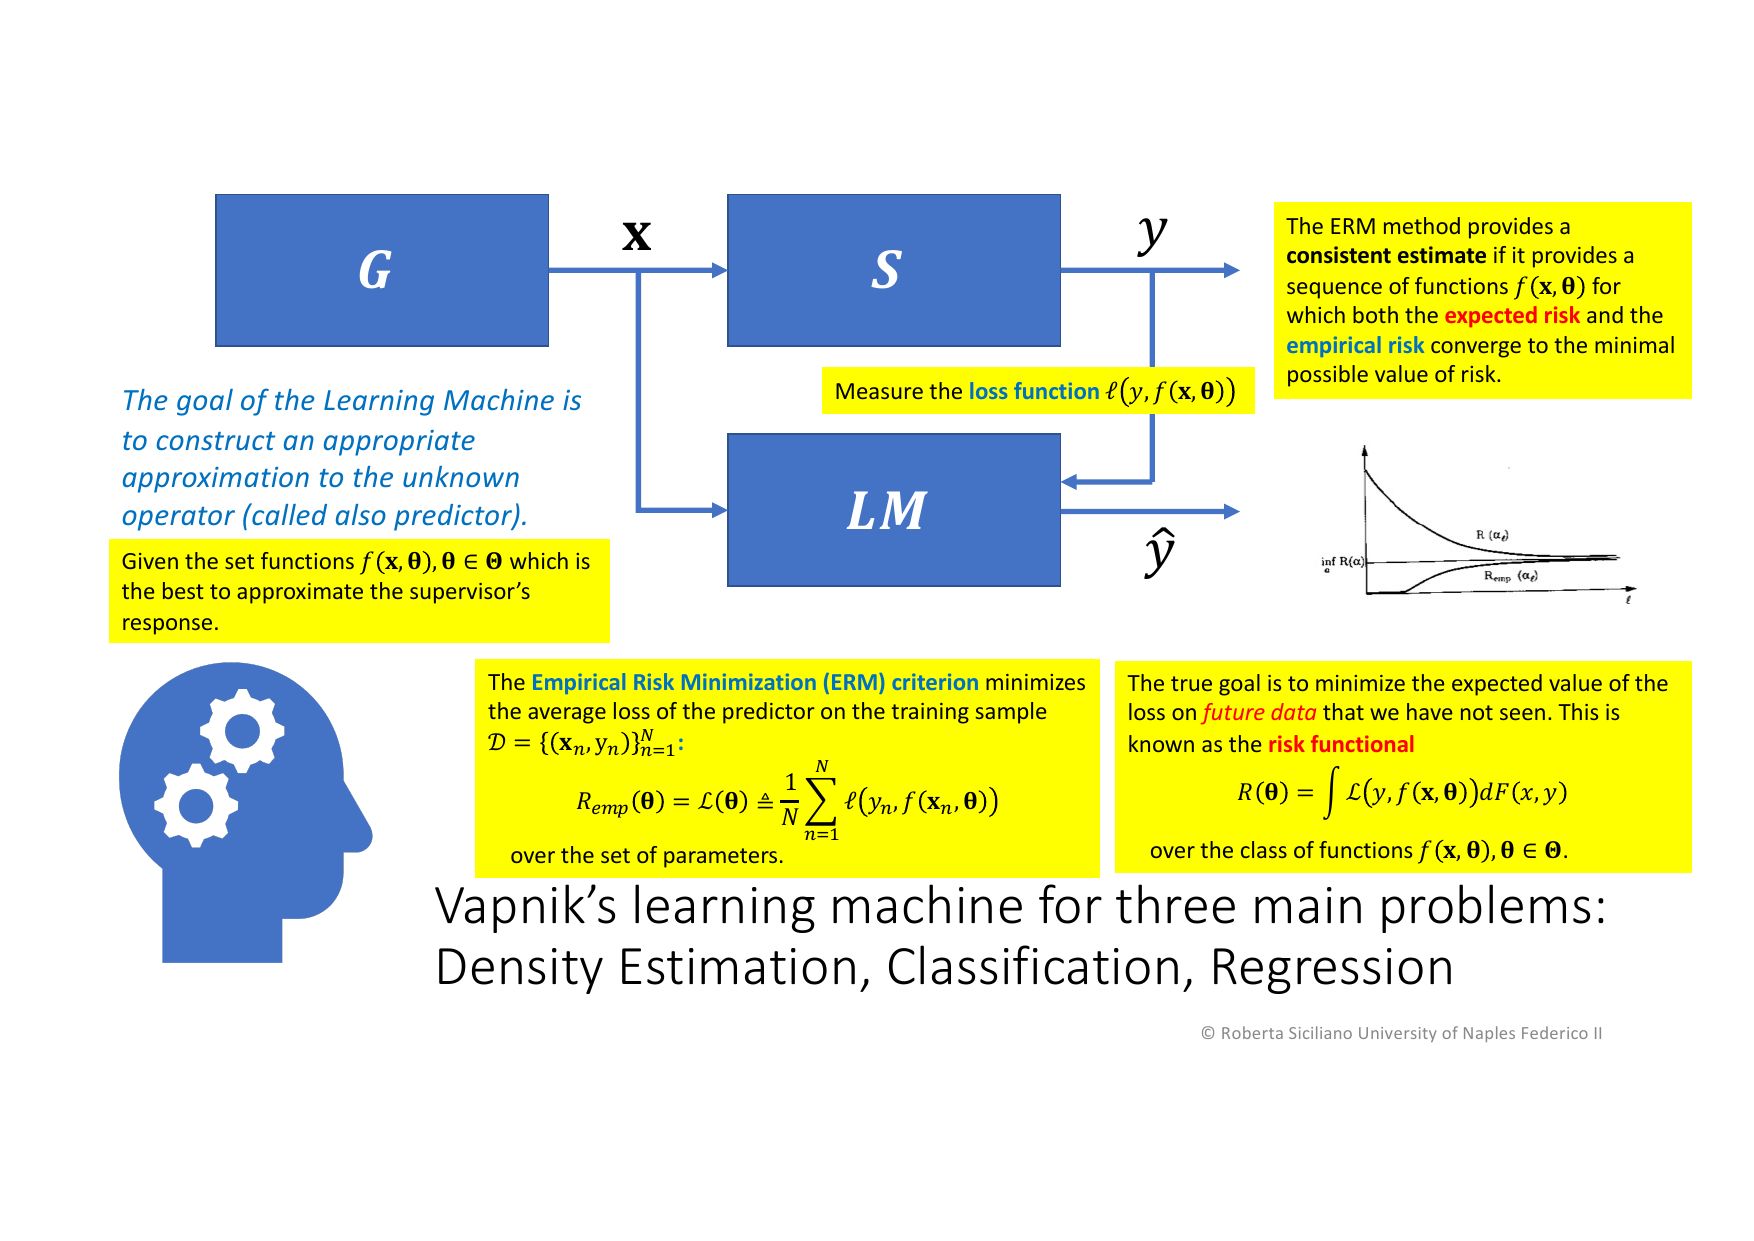
\includegraphics[width=0.85\textwidth]{slide_028}
    \caption{Vapnik's ERM scheme: the LM compares its prediction $\hat y$ against the supervisor's answer $y$ via the loss function; as more data arrive, both the empirical risk $R_{\text{emp}}$ and the expected risk $R$ converge towards the smallest achievable risk.}
    \captionsetup{font=footnotesize}
\end{figure}

\begin{noteboxtitle}{Three classical problems}
Vapnik's learning-machine framework was built to unify three main statistical problems, which the next slides go through in turn: \textbf{Density Estimation}, \textbf{Regression}, and \textbf{Classification}. What changes between them is simply the choice of loss function $\ell(\cdot,\cdot)$.
\end{noteboxtitle}

\subsection{Density Estimation, Regression, and Regression Estimation}\label{sec:rl-prolusion-density-regression}

\subsubsection{Density estimation (Fisher-Wald setting)}

Sometimes we are not trying to predict an output at all — we simply want to describe how the data $\mathbf{x}$ are distributed. This is \textbf{density estimation}: we look for the best density $p(\mathbf{x}, \boldsymbol\theta)$, among a family indexed by $\boldsymbol\theta \in \boldsymbol\Theta$, that fits the observed data.

The natural loss function here is the negative log-density:
\[
  L\bigl(y, p(\mathbf{x}, \boldsymbol\theta)\bigr) = -\log p(\mathbf{x}, \boldsymbol\theta)
\]
\begin{itemize}
  \item $p(\mathbf{x}, \boldsymbol\theta)$: the candidate density, evaluated at the observed point $\mathbf{x}$.
  \item The minus sign in front of the logarithm turns ``high probability'' into ``low loss'': a density that assigns high probability to the data we actually observed pays a small penalty.
\end{itemize}
\textit{Intuition: the best density is the one that makes the data we observed look as likely as possible — this is exactly the idea behind maximum likelihood.}

The density that minimizes the risk functional with this loss is exactly the desired density; the estimation problem is to minimize the risk knowing only i.i.d.\ samples, without knowing $p(y \mid \mathbf{x})$ in advance.

\subsubsection{Regression}

\textbf{Regression} deals with predicting a continuous, real-valued output. Typical applications: economic assets (revenue, cost, production), chemical/biological/geological measurements, astrophysics, and so on.

A regression algorithm typically returns:
\begin{itemize}
  \item a predicted \textbf{response value},
  \item a \textbf{standard deviation} (how uncertain the prediction is),
  \item the \textbf{Mean Squared Error} (how well the model fits overall).
\end{itemize}

\subsubsection{Regression estimation}

Let the supervisor's answer $y$ now be a real number, and let $f(\mathbf{x}, \boldsymbol\theta)$, $\boldsymbol\theta \in \boldsymbol\Theta$, be a family of real-valued functions that contains the true regression function
\[
  f(\mathbf{x}, \theta_0) = \int y \, dF(y \mid x).
\]
\begin{itemize}
  \item $f(\mathbf{x}, \theta_0)$: the (unknown) true regression function — the average value of $y$ given $\mathbf{x}$, according to the true conditional distribution $F(y\mid x)$.
\end{itemize}
\textit{Intuition: the ``true'' regression curve is simply the conditional mean of $y$ given $\mathbf{x}$ — on average, what $y$ tends to be for a given $\mathbf{x}$.}

The regression function is exactly the one that minimizes the risk functional under the \textbf{squared loss}:
\[
  L\bigl(y, f(\mathbf{x}, \boldsymbol\theta)\bigr) = \bigl(y - f(\mathbf{x}, \boldsymbol\theta)\bigr)^2
\]
\begin{itemize}
  \item $y - f(\mathbf{x}, \boldsymbol\theta)$: the prediction error (residual) for one example.
  \item Squaring it makes big errors count much more than small ones, and removes the sign.
\end{itemize}
\textit{Intuition: this is exactly the familiar least-squares idea — the further off a prediction is, the more heavily it is penalized (quadratically).}

So regression estimation means: minimize the risk functional $R(\boldsymbol\theta)$ with the squared loss, in the realistic situation where $p(y\mid \mathbf{x})$ is unknown and only sample data $\mathcal{D}$ are available.

\subsection{Classification, the Iris Dataset, and Uncertainty}\label{sec:rl-prolusion-classification}

\subsubsection{Data classification}

\textbf{Classification} deals with predicting a categorical output (a label). Typical applications: customer target marketing, medical disease outcome, document categorization (e.g.\ spam filtering), multimedia categorization, image classification, face detection, and many more.

A classification algorithm typically provides:
\begin{itemize}
  \item a \textbf{label prediction}: assign a new instance to one class;
  \item a \textbf{numerical score}: a propensity (a number) reflecting how confident the model is that an instance belongs to a class, useful for ranking instances;
  \item an \textbf{error rate}: how often the model gets it wrong.
\end{itemize}

\subsubsection{Formalizing classification}

The output space is a set of $C$ unordered, mutually exclusive labels, $y \in \{1, 2, \dots, C\}$.
\begin{itemize}
  \item \textbf{Binary} classification if $C = 2$ (commonly coded as $y \in \{0,1\}$ or $y \in \{-1,+1\}$).
  \item \textbf{Multi-class} classification if $C > 2$.
\end{itemize}

Taking $C=2$ with $y \in \{0,1\}$, performance on the training set is often measured with the \textbf{misclassification rate}:
\[
  \mathcal{L}(\boldsymbol\theta) \triangleq \frac{1}{N}\sum_{n=1}^{N} I\bigl(y_n \neq f(\mathbf{x}_n; \boldsymbol\theta)\bigr) =
  \begin{cases}
    0 & \text{if } y_n = f(\mathbf{x}_n; \boldsymbol\theta) \\
    1 & \text{if } y_n \neq f(\mathbf{x}_n; \boldsymbol\theta)
  \end{cases}
\]
\begin{itemize}
  \item $I(\cdot)$: the indicator function, which is $1$ when the condition inside is true (a mistake was made) and $0$ otherwise.
\end{itemize}
\textit{Intuition: this is simply the fraction of examples the model got wrong — it treats every mistake as equally bad.}

\begin{noteboxtitle}{Not all errors are equal}
In practice some mistakes cost more than others (e.g.\ missing a disease diagnosis is worse than a false alarm). An \textbf{asymmetric loss function} can assign different costs to different kinds of errors. The general Empirical Risk definition $\mathcal{L}(\boldsymbol\theta) \triangleq \frac{1}{N}\sum_{n=1}^N \ell(y_n, f(\mathbf{x}_n, \boldsymbol\theta))$ covers this: the misclassification rate above is just the special case where every error costs exactly $1$.
\end{noteboxtitle}

\subsubsection{Fisher's Iris dataset}

\vs
\begin{example}[The Iris flower dataset (1936)]
Ronald Fisher's Iris dataset is the classic toy example for classification: $50$ samples from each of \textbf{three species} of iris (\textit{setosa}, \textit{versicolor}, \textit{virginica}), so $N = 150$ in total. Each flower is described by $4$ numeric features: sepal length, sepal width, petal length, petal width (all in cm). Fisher used a \textbf{linear discriminant model} to separate the three species based on these four measurements — one of the very first classification algorithms in statistics.
\end{example}

\begin{figure}[H]
    \centering
    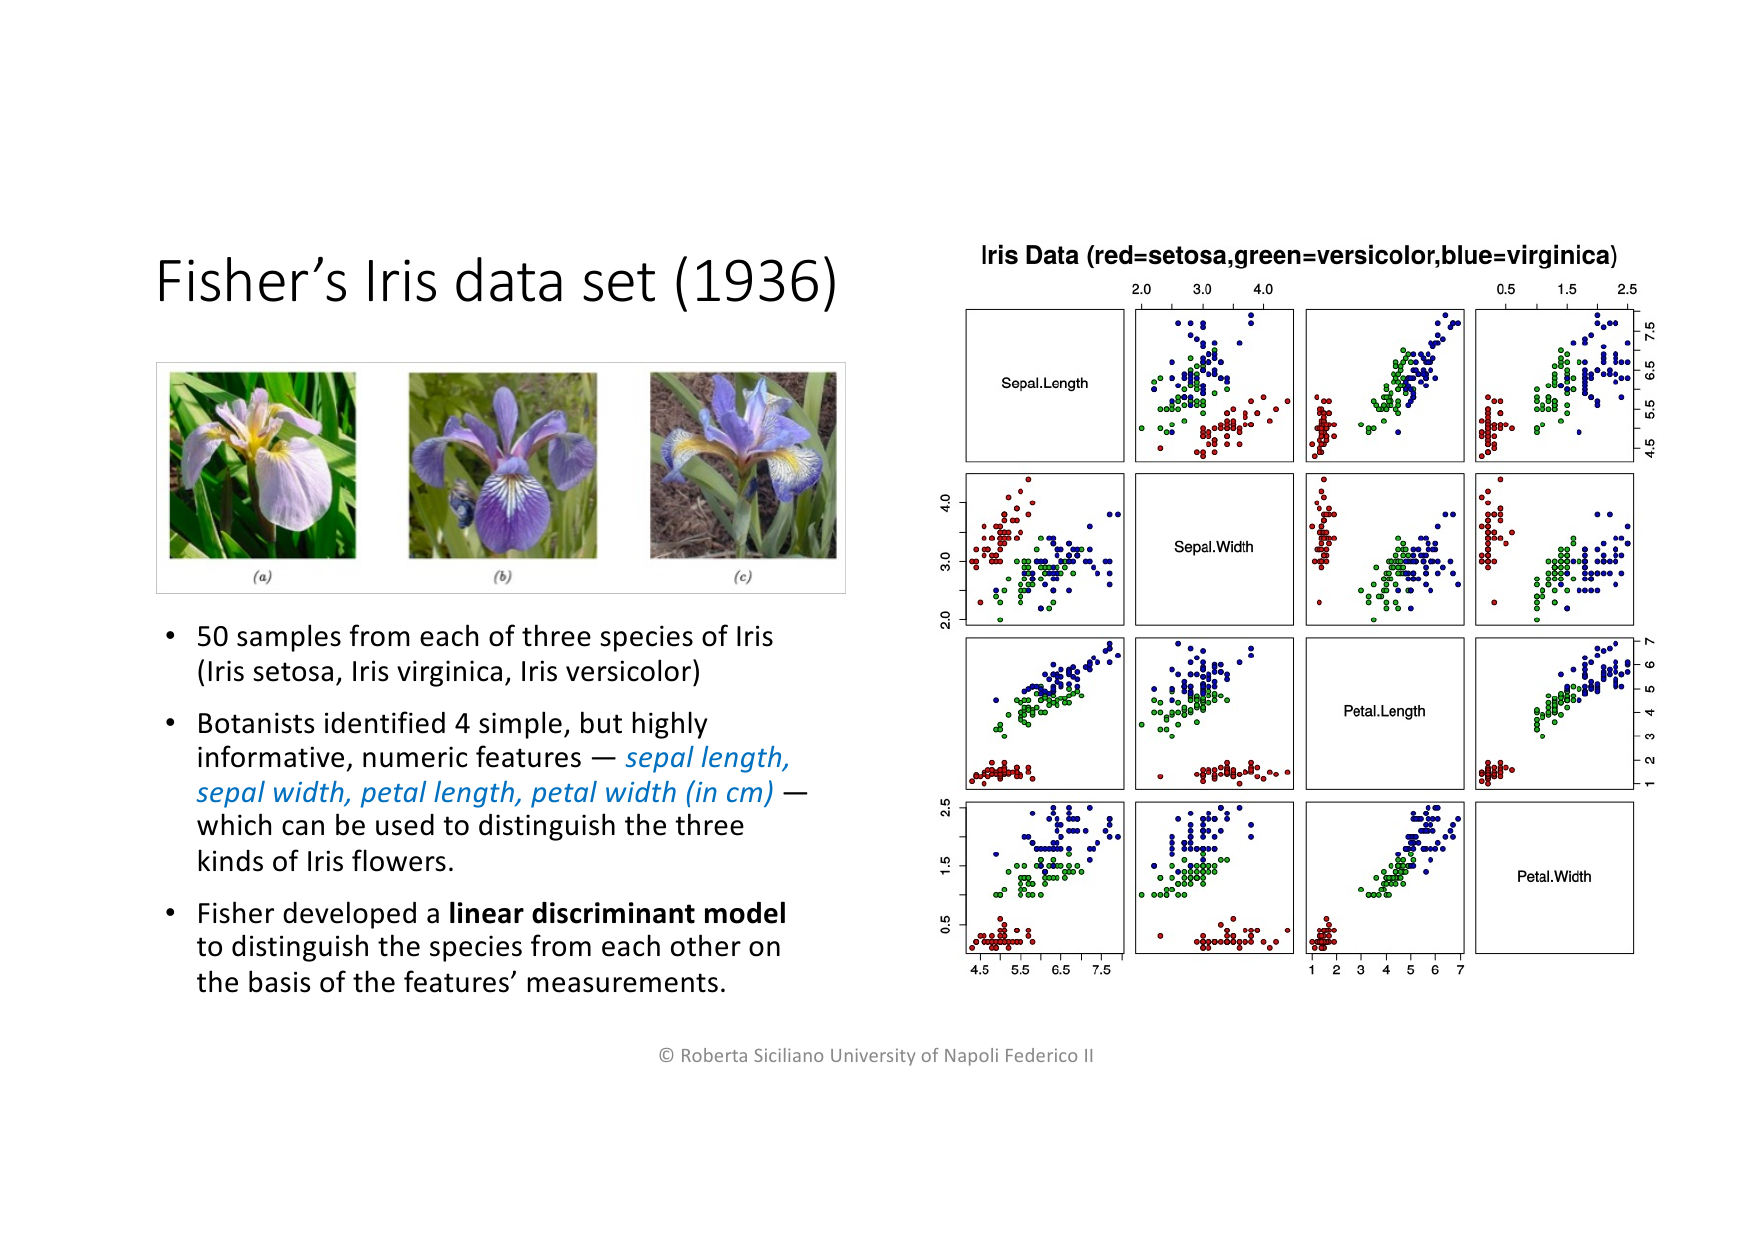
\includegraphics[width=0.85\textwidth]{slide_033}
    \caption{The three Iris species and pairwise scatterplots of the four features, colored by species.}
    \captionsetup{font=footnotesize}
\end{figure}

Petal length and petal width alone already separate the three species reasonably well, which is why a simple decision tree does a good job on this dataset (see Figure~\ref{fig:rl-iris-analysis}).

\begin{figure}[H]
    \centering
    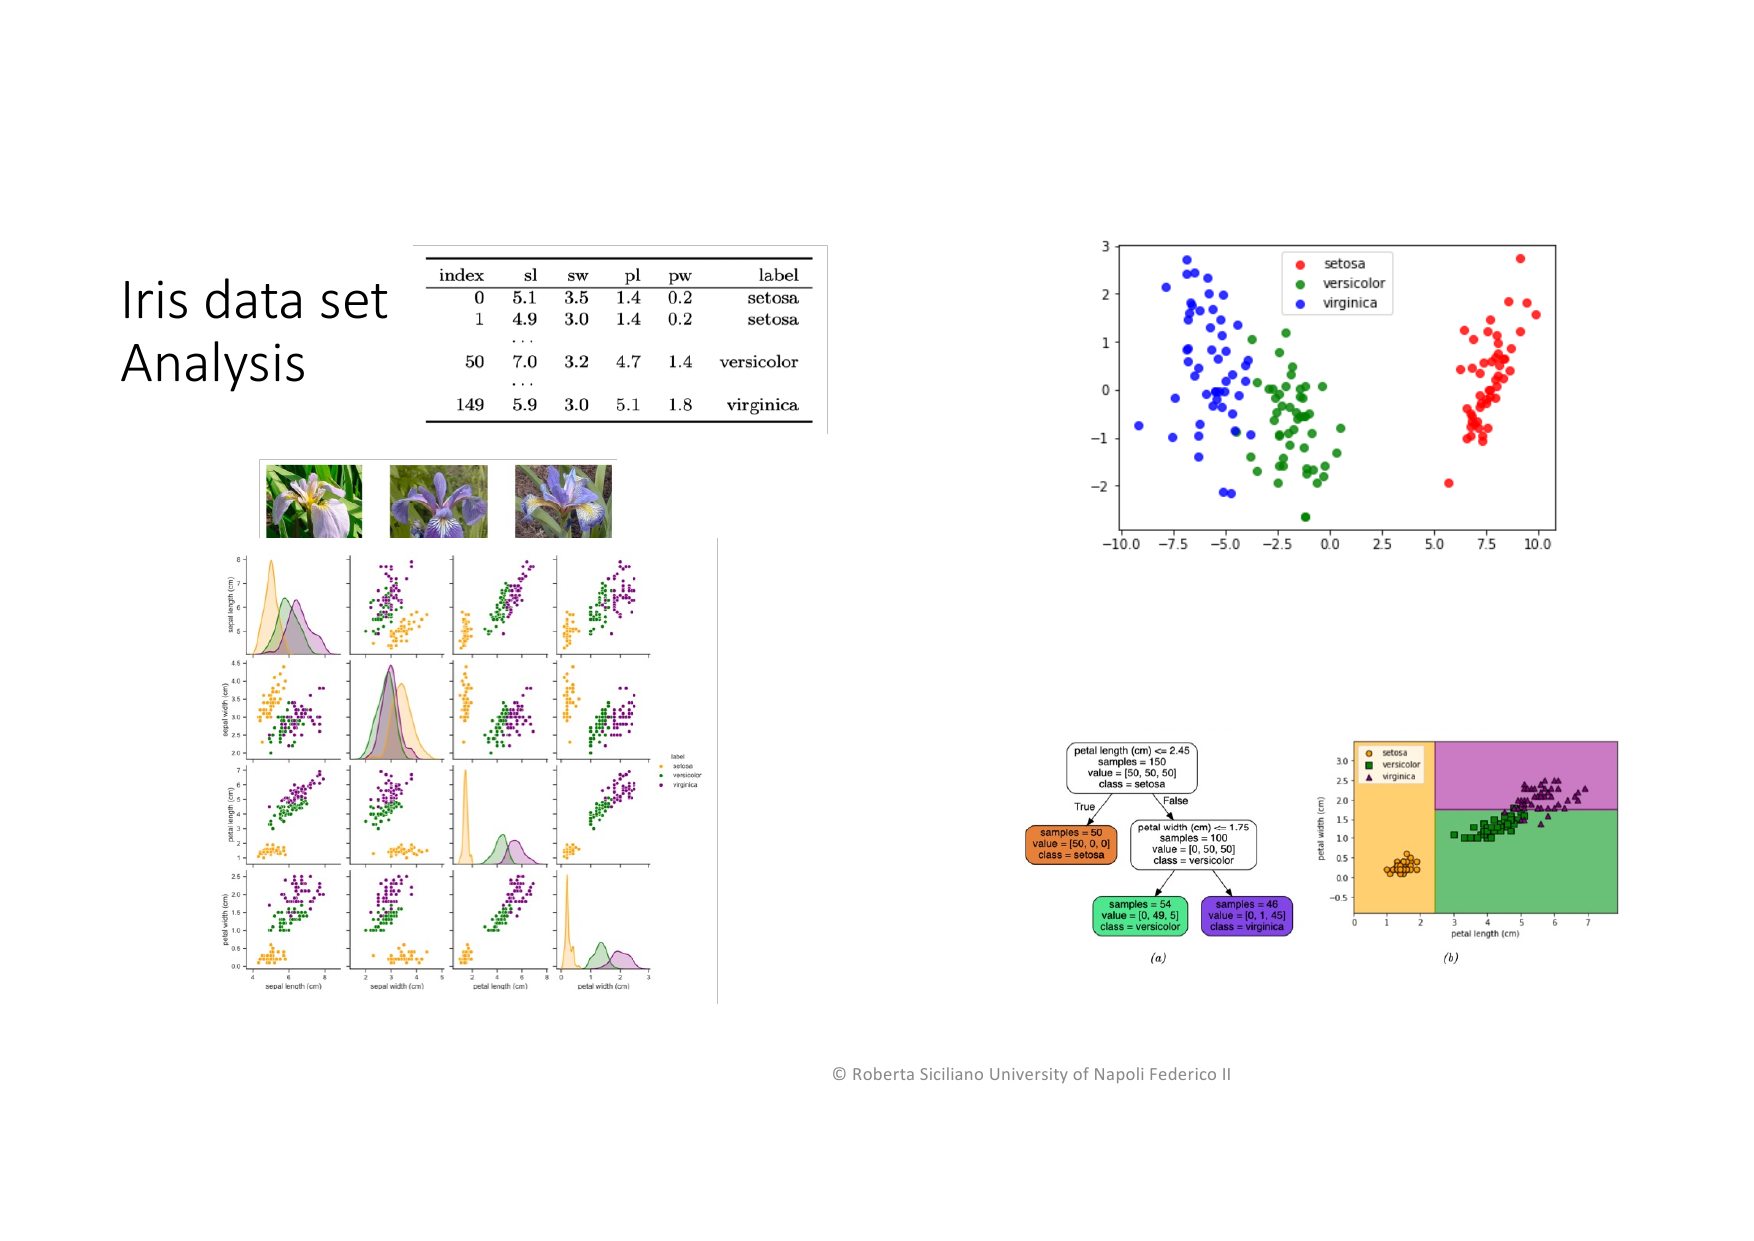
\includegraphics[width=0.85\textwidth]{slide_034}
    \label{fig:rl-iris-analysis}
    \caption{Iris data table, pairwise scatterplots with class densities on the diagonal, a linear-discriminant-style projection, and a decision tree with its resulting decision regions in the (petal length, petal width) plane.}
    \captionsetup{font=footnotesize}
\end{figure}

\begin{example}[Classifying Iris with scikit-learn]
\vs
\begin{lstlisting}[language=Python, caption={A minimal classifier on the Iris dataset}]
from sklearn.datasets import load_iris
from sklearn.model_selection import train_test_split
from sklearn.tree import DecisionTreeClassifier
from sklearn.metrics import accuracy_score

X, y = load_iris(return_X_y=True)
X_train, X_test, y_train, y_test = train_test_split(
    X, y, test_size=0.3, random_state=0)

clf = DecisionTreeClassifier(max_depth=3, random_state=0)
clf.fit(X_train, y_train)

y_pred = clf.predict(X_test)
print("Accuracy:", accuracy_score(y_test, y_pred))
\end{lstlisting}
This is the kind of small, self-contained snippet you could adapt for a homework exercise: load the data, split it, fit a classifier, measure the misclassification rate on held-out data.
\end{example}

\subsubsection{Uncertainty in classification}

Even a good classifier is rarely $100\%$ certain, because $p(y \mid \mathbf{x})$ is unknown and only sample data are available. We can express our uncertainty using a conditional probability distribution over the classes:
\[
  p(y = c \mid \mathbf{x}, \boldsymbol\theta) = f_c(\mathbf{x}, \boldsymbol\theta), \qquad c \in C.
\]
\begin{itemize}
  \item $f_c(\mathbf{x}, \boldsymbol\theta)$: the model's estimated probability that the true class is $c$, given input $\mathbf{x}$.
\end{itemize}
\textit{Intuition: instead of a single guess, the model returns a probability for each possible class (e.g.\ 80\% setosa, 15\% versicolor, 5\% virginica).}

When fitting probabilistic models it is common to use the \textbf{negative log probability} as the loss:
\[
  \ell\bigl(y, f(\mathbf{x}, \boldsymbol\theta)\bigr) = -\log p(y \mid \mathbf{x}, \boldsymbol\theta).
\]
A good model (low loss) assigns a high probability to the true label $y$ for each input $\mathbf{x}$. Averaging this loss over the whole training set gives the \textbf{Negative Log-Likelihood (NLL)}:
\[
  NLL(\boldsymbol\theta) = -\frac{1}{N}\sum_{n=1}^{N} \log p(y_n \mid \mathbf{x}_n, \boldsymbol\theta).
\]
\begin{itemize}
  \item $N$: number of training examples; $n$: index over them.
\end{itemize}
\textit{Intuition: minimizing the NLL means finding the parameters $\boldsymbol\theta$ that make the observed labels as probable as possible under the model — exactly the maximum-likelihood principle, now dressed up as a loss function to minimize.}

\subsubsection{Model uncertainty versus data uncertainty}

It is useful to separate \emph{why} a prediction might be wrong. This assumes there is a ``true'' model generating the data and a genuinely ``best'' way to analyze it.

\begin{itemize}
  \item \textbf{Model uncertainty} (epistemic uncertainty) comes from a \emph{lack of knowledge} about the true input-output mapping — also called model specification error. It is often due to too little training data. Examples: an under-represented minority class in a face-recognition dataset, or rare words in a language model.
  \item \textbf{Data uncertainty} comes from intrinsic, irreducible randomness in the mapping itself. It refers to the variation coming from the error term, a random variable that is uncorrelated with the predictors and has mean zero. The predictor captures the systematic information the inputs provide about the target; if the inputs carry no information at all, the predictor just returns the average output.
\end{itemize}
\textit{Intuition: model uncertainty is ``we haven't learned enough yet'' (fixable with more/better data); data uncertainty is ``the world is inherently noisy'' (never fully fixable, no matter how much data we collect).}

\subsection{Overview of Supervised Models and the No Free Lunch Theorem}\label{sec:rl-prolusion-nfl}

\subsubsection{A map of supervised learning models}

There are many families of supervised learning algorithms, ranging from simple linear methods to highly flexible, non-linear ones.

\begin{figure}[H]
    \centering
    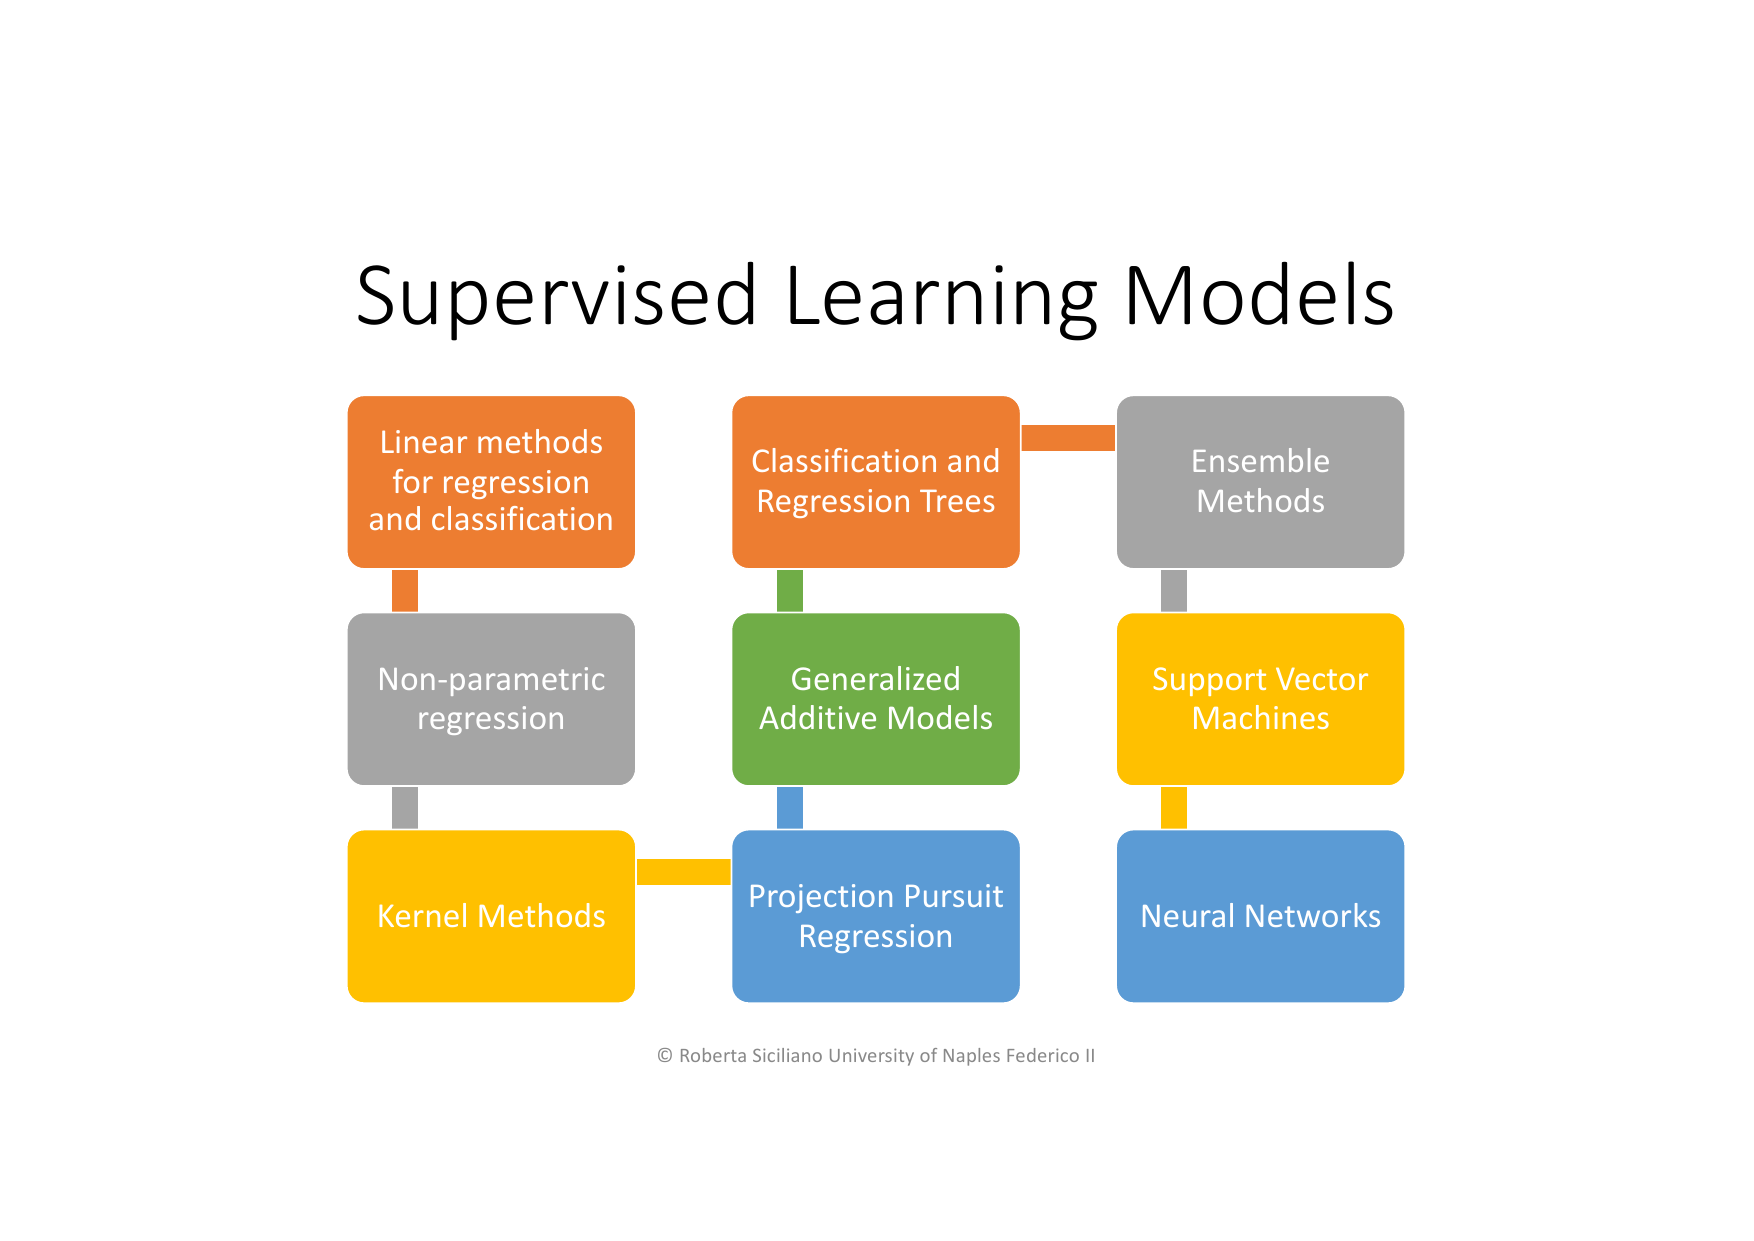
\includegraphics[width=0.85\textwidth]{slide_038}
    \caption{A map of supervised learning models: linear methods, non-parametric regression, kernel methods, classification and regression trees, generalized additive models, projection pursuit regression, ensemble methods, support vector machines, and neural networks.}
    \captionsetup{font=footnotesize}
\end{figure}

These families differ in flexibility, interpretability, and how they trade off bias and variance — several of them will be studied in detail later in the course.

\subsubsection{No Free Lunch theorem}

\begin{noteboxtitle}{``All Models Are Wrong''}
George Box (1976): \textit{``All models are wrong, but some are useful. Some are more wrong than others, some may be harmful.''}
\end{noteboxtitle}

The \textbf{No Free Lunch theorem} states that \textbf{no single method dominates all others across every possible dataset}. There is no universally best algorithm: which model works best depends on the specific problem and data at hand. Selecting the right approach for the task is therefore one of the biggest practical challenges in statistical/machine learning — in short, \textit{``there is no free lunch in statistics''}.

\begin{figure}[H]
    \centering
    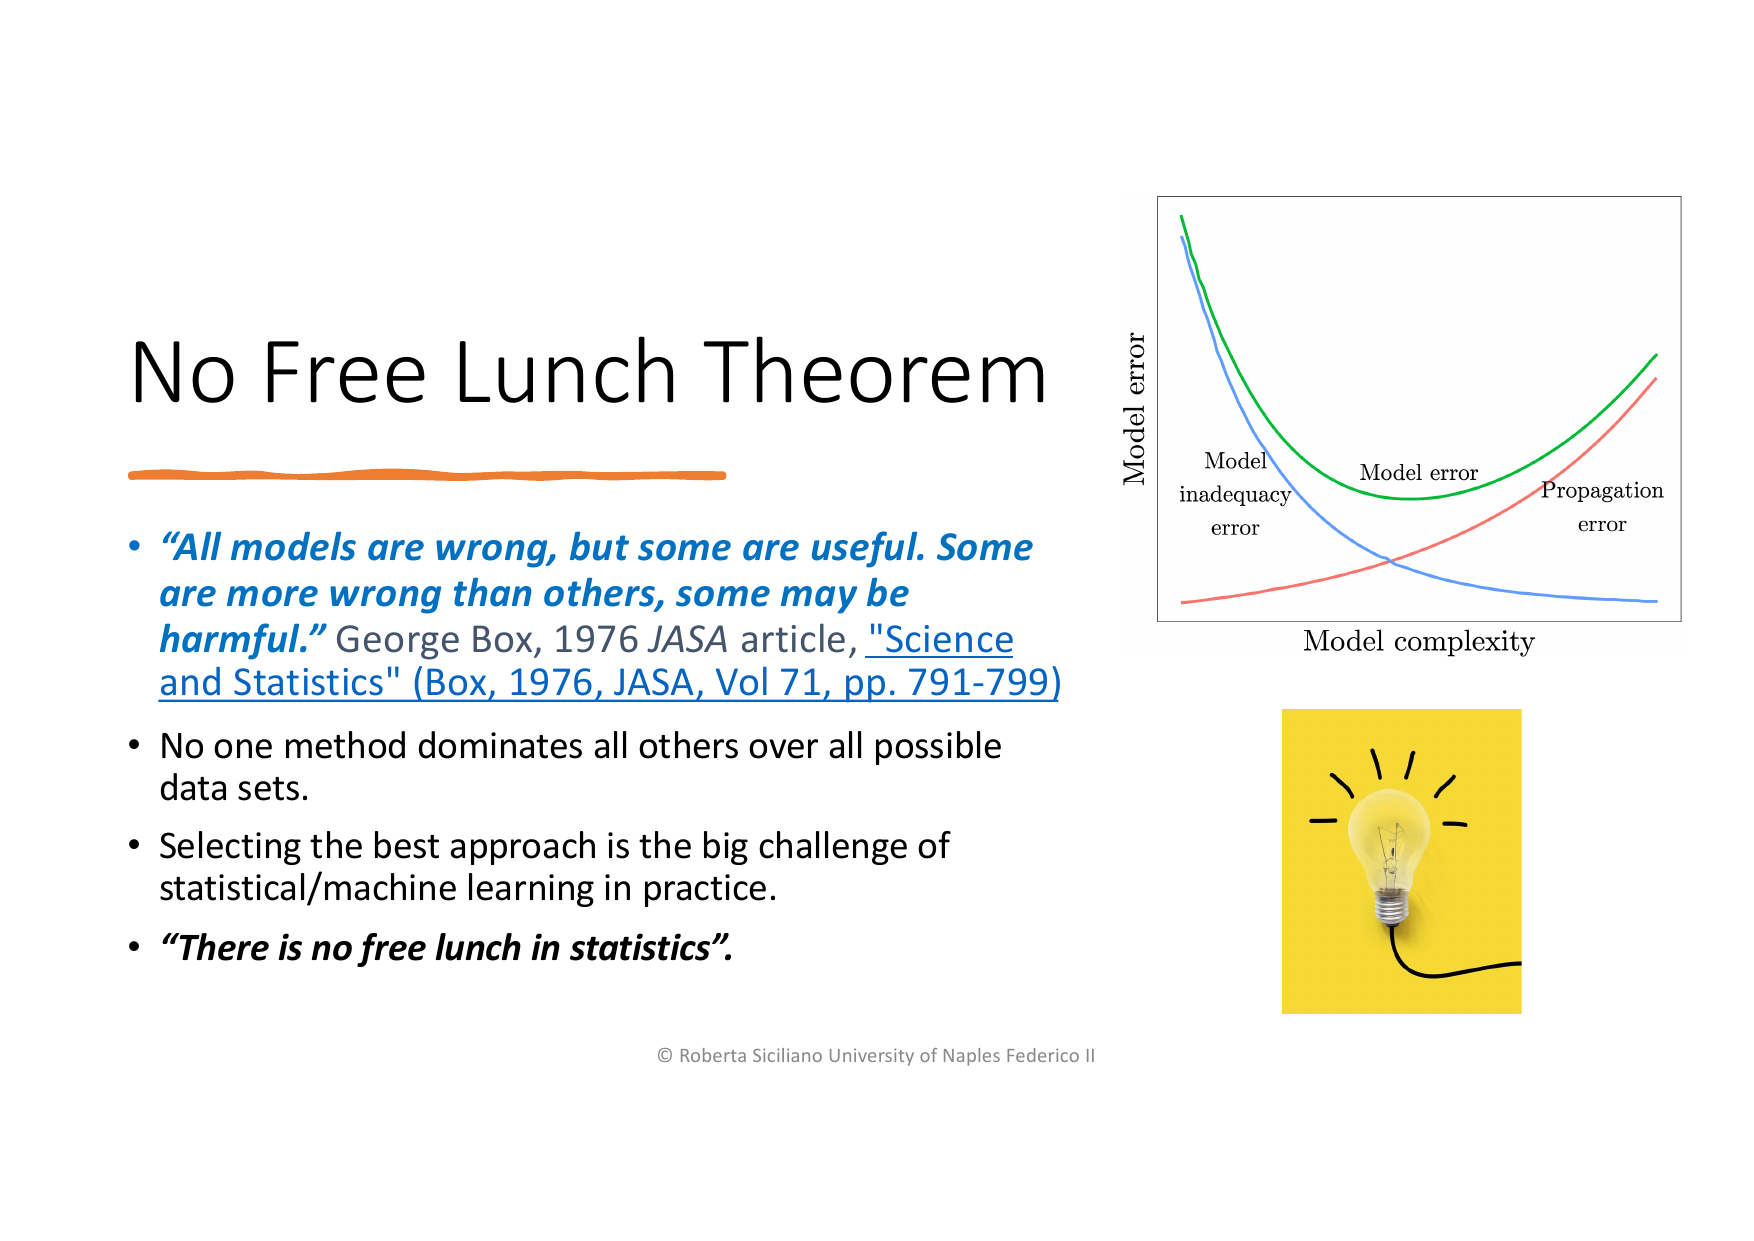
\includegraphics[width=0.60\textwidth]{slide_039}
    \caption{Model error as a function of model complexity: inadequacy error decreases while propagation error increases with complexity, producing a U-shaped total model error curve with an optimal complexity in between.}
    \captionsetup{font=footnotesize}
\end{figure}

\textit{Intuition: a model that is too simple underfits (large ``model inadequacy'' error), while a model that is too complex overfits and propagates noise (large ``propagation'' error); the best model complexity sits at the bottom of the U-shaped curve.}

\subsection{What is Reinforcement Learning?}\label{sec:rl-intro-what-is-rl}

So far we have talked about supervised learning (learning from labelled examples)
and unsupervised learning (finding structure without labels). \textbf{Reinforcement
Learning (RL)} is a third, very different way of learning: an agent learns by
\textit{doing}, not by being shown the right answer.

\subsubsection{The agent-environment loop}

\begin{defbox}{Reinforcement Learning}
The problem RL tries to solve is: find suitable \textbf{actions} to take in a given
situation in order to maximize a \textbf{reward}.

\textit{Think of it like training a dog to do a trick}: you don't give the dog a
rulebook, you just give it a treat when it does something close to what you want,
and nothing (or a scolding) when it doesn't. Over many attempts, the dog figures
out, by trial and error, which sequence of movements leads to the treat.
\end{defbox}

The picture is always the same: an \textbf{agent} (the learner/decision-maker) sits
inside an \textbf{environment} (everything it interacts with). At each time step $t$:
\begin{itemize}
  \item the agent observes the current \textbf{state} $s_t$ of the environment,
  \item it chooses an \textbf{action} $a_t$,
  \item the environment responds with a \textbf{reward} $r_t$ and moves to a new
        state $s_{t+1}$ (\textit{state transition}).
\end{itemize}

\begin{figure}[H]
    \centering
    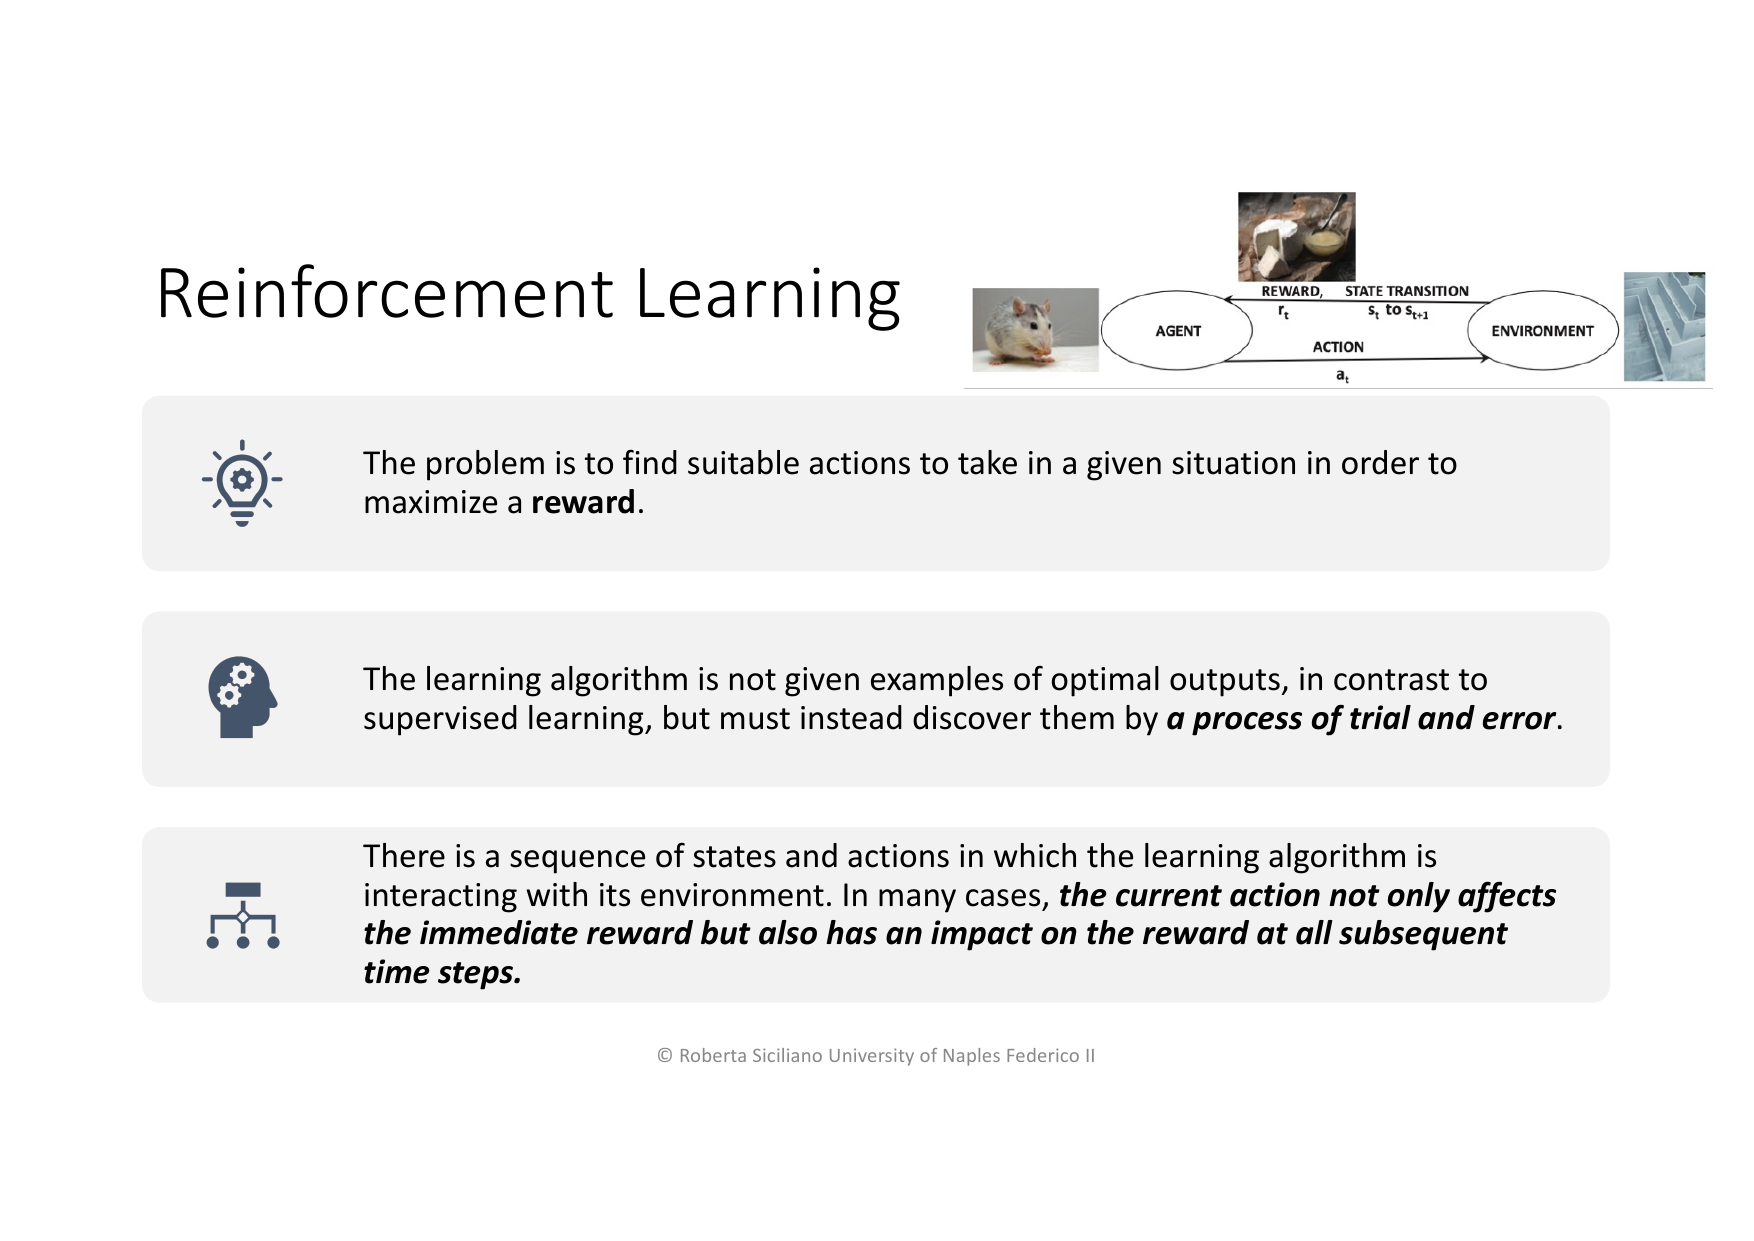
\includegraphics[width=0.85\textwidth]{slide_040}
    \caption{Agent-environment interaction loop: the agent takes an action, the environment returns a reward and the next state.}
    \captionsetup{font=footnotesize}
\end{figure}

This loop repeats over and over, and the agent's only goal is to pick actions that
make the total reward as large as possible over time -- not just the reward at the
very next step.

\subsubsection{Learning by trial and error, not by examples}

The key difference from supervised learning is that \textbf{nobody tells the agent
what the correct action is}. In supervised learning, every training example comes
with the right label attached. In RL, the algorithm is never handed ``the optimal
move'' -- it has to discover good actions itself, \textit{by a process of trial and
error}: try something, see what reward comes back, and adjust.

\textit{Analogy}: think of a robot learning to walk. Nobody gives it a table of
``correct'' joint angles for every possible position. Instead, it tries moving its
legs, sometimes it falls (low/negative reward), sometimes it takes a step forward
without falling (positive reward), and slowly, over thousands of attempts, it
learns a walking pattern that keeps it upright and moving.

\subsubsection{Actions have long-term consequences}

\begin{noteboxtitle}{Watch out}
There is a sequence of states and actions in which the agent keeps interacting
with its environment. In many cases, \textit{the current action not only affects
the immediate reward but also has an impact on the reward at all subsequent time
steps.}
\end{noteboxtitle}

This is what makes RL genuinely harder than a simple ``guess and check'' problem:
an action that looks bad right now (e.g. moving away from the treat) might be
exactly what sets up a big reward later (e.g. positioning yourself to grab it).
The agent has to reason about the future, not just the present.

\vs
\begin{example}[Chess as an RL problem]
Think of an agent learning to play chess purely by playing games against itself.
\begin{itemize}
  \item \texttt{State:} the current configuration of the board.
  \item \texttt{Action:} a legal move.
  \item \texttt{Reward:} essentially zero for most moves, and $+1$/$-1$ only at
        the end of the game (win/lose).
\end{itemize}
Notice how a single opening move can influence the outcome dozens of moves later --
exactly the ``delayed consequences'' problem described above.
\end{example}

\subsection{Exploration versus Exploitation}\label{sec:rl-intro-exploration-exploitation}

Once the agent has tried a few actions and has some idea of what works, it faces a
dilemma that is central to all of RL.

\begin{defbox}{Exploration vs.\ Exploitation}
\textbf{Exploitation}: the agent uses the actions it already knows to yield a high
reward -- it plays it safe and sticks to what has worked before.

\textbf{Exploration}: the agent tries out new, untested actions just to see how
effective they are -- it takes a risk to gather more information.

\textit{Reinforcement learning requires dealing with the trade-off between the two:
focusing too strongly on either exploration or exploitation alone will yield poor
results.}
\end{defbox}

\textit{Analogy}: imagine you always order the same dish at your favourite
restaurant because you know you'll enjoy it (exploitation). You will never
discover that the dish on the other side of the menu is even better, unless you
occasionally take the risk of trying something new (exploration). But if you
never repeat a dish you liked, you also never get to actually enjoy your
favourite meal. RL agents face exactly this dilemma at every single step.

\subsubsection{Why the dilemma cannot be avoided}

\begin{itemize}
  \item The agent must try a variety of actions and progressively favor the ones
        that appear best -- but ``appear best'' is based on limited experience.
  \item On a stochastic (random/noisy) task, a single good result from an action
        could be luck: each action must be tried many times to get a reliable
        estimate of its \textit{expected reward}.
  \item Neither pure exploration (never using what you've learned) nor pure
        exploitation (never trying anything new) works: the dilemma is that
        neither one can be pursued exclusively without failing at the task.
\end{itemize}

In practice, a common strategy (seen later in the course, e.g.\ $\varepsilon$-greedy
methods) is to explore a lot early on, and gradually shift towards exploitation as
the agent becomes more confident about which actions are good.

\subsection{RL as the Gateway to General AI}\label{sec:rl-intro-gateway-general-ai}

RL is not just one more algorithm among many: it tackles the \textbf{whole}
problem of an agent acting in the world, rather than a small isolated
sub-problem.

\subsubsection{Simple to judge, hard to specify}

Many real tasks share a common feature: it is easy to tell if the outcome is good,
but very hard to write down a rule for how to achieve it, and it's cheap to
generate trial-and-error data for them. Typical examples: video games (e.g.\
Atari), board and card games (chess, Go, poker), \textbf{robot locomotion and
visuomotor skills}, and \textbf{self-driving cars}. In all of these you can easily
say ``the robot fell over'' or ``the car crashed'', but writing an explicit
rulebook for ``how to walk'' or ``how to drive'' is extremely hard -- much easier
to let the agent discover it through experience.

\subsubsection{A goal-directed agent in an uncertain world}

\begin{noteboxtitle}{The bigger picture}
A key feature of RL is that it considers the \textit{whole} problem of a
goal-directed agent interacting with an uncertain environment, instead of
breaking the problem into isolated sub-tasks and hoping they add up to
intelligent behaviour.

All RL agents share three ingredients: they have \textbf{explicit goals}, they can
\textbf{sense} aspects of their environment, and they can \textbf{choose actions}
to influence that environment.
\end{noteboxtitle}

This complete, interactive, goal-seeking picture is precisely why RL is often
described as \textbf{the gateway to general forms of artificial intelligence}: it
is the closest existing framework to how a truly autonomous agent -- one that
perceives, decides, and acts to pursue a goal -- would have to operate.

\subsection{Recap: Statistical Learning Trade-Offs}\label{sec:rl-intro-recap-tradeoffs}

Before moving into the technical part of the course, it is useful to see the full
map of trade-offs that statistical/machine learning revolves around -- several of
which have already been discussed in earlier parts of the course, and the last
one is exactly what we just introduced above.

\begin{itemize}
  \item Supervised \textit{versus} Unsupervised Learning.
  \item Regression \textit{versus} Classification problem.
  \item Parametric \textit{versus} Non-parametric methods.
  \item \textit{Trade-off} between Accuracy and Interpretability.
  \item Bias-Variance \textit{Trade-off}.
  \item Trade-off Exploration \textit{versus} Exploitation.
\end{itemize}

The first five were the subject of earlier parts of the course (see
Section~\ref{sec:sl-foundations} and the unsupervised learning material); the last
one, Exploration vs.\ Exploitation, is the trade-off specific to Reinforcement
Learning that we just introduced in
Section~\ref{sec:rl-intro-exploration-exploitation}.

\subsection{Course Logistics}\label{sec:rl-intro-course-logistics}

The remaining slides are organisational information about the course rather than
theory -- useful as a reference, summarised briefly here.

\subsubsection{Road map}

The course (Module A) moves from the probabilistic foundations of ML, through
Bayesian and generative models, into Reinforcement Learning proper: starting with
Q-Learning, then Deep Q-Learning (DQN), SARSA, policy-gradient methods (REINFORCE,
Actor-Critic), and finally more advanced algorithms (PPO, DDPG, Soft Actor-Critic)
before covering the Exploration vs.\ Exploitation / Multi-Arm Bandits topic and
the exam.

\begin{figure}[H]
    \centering
    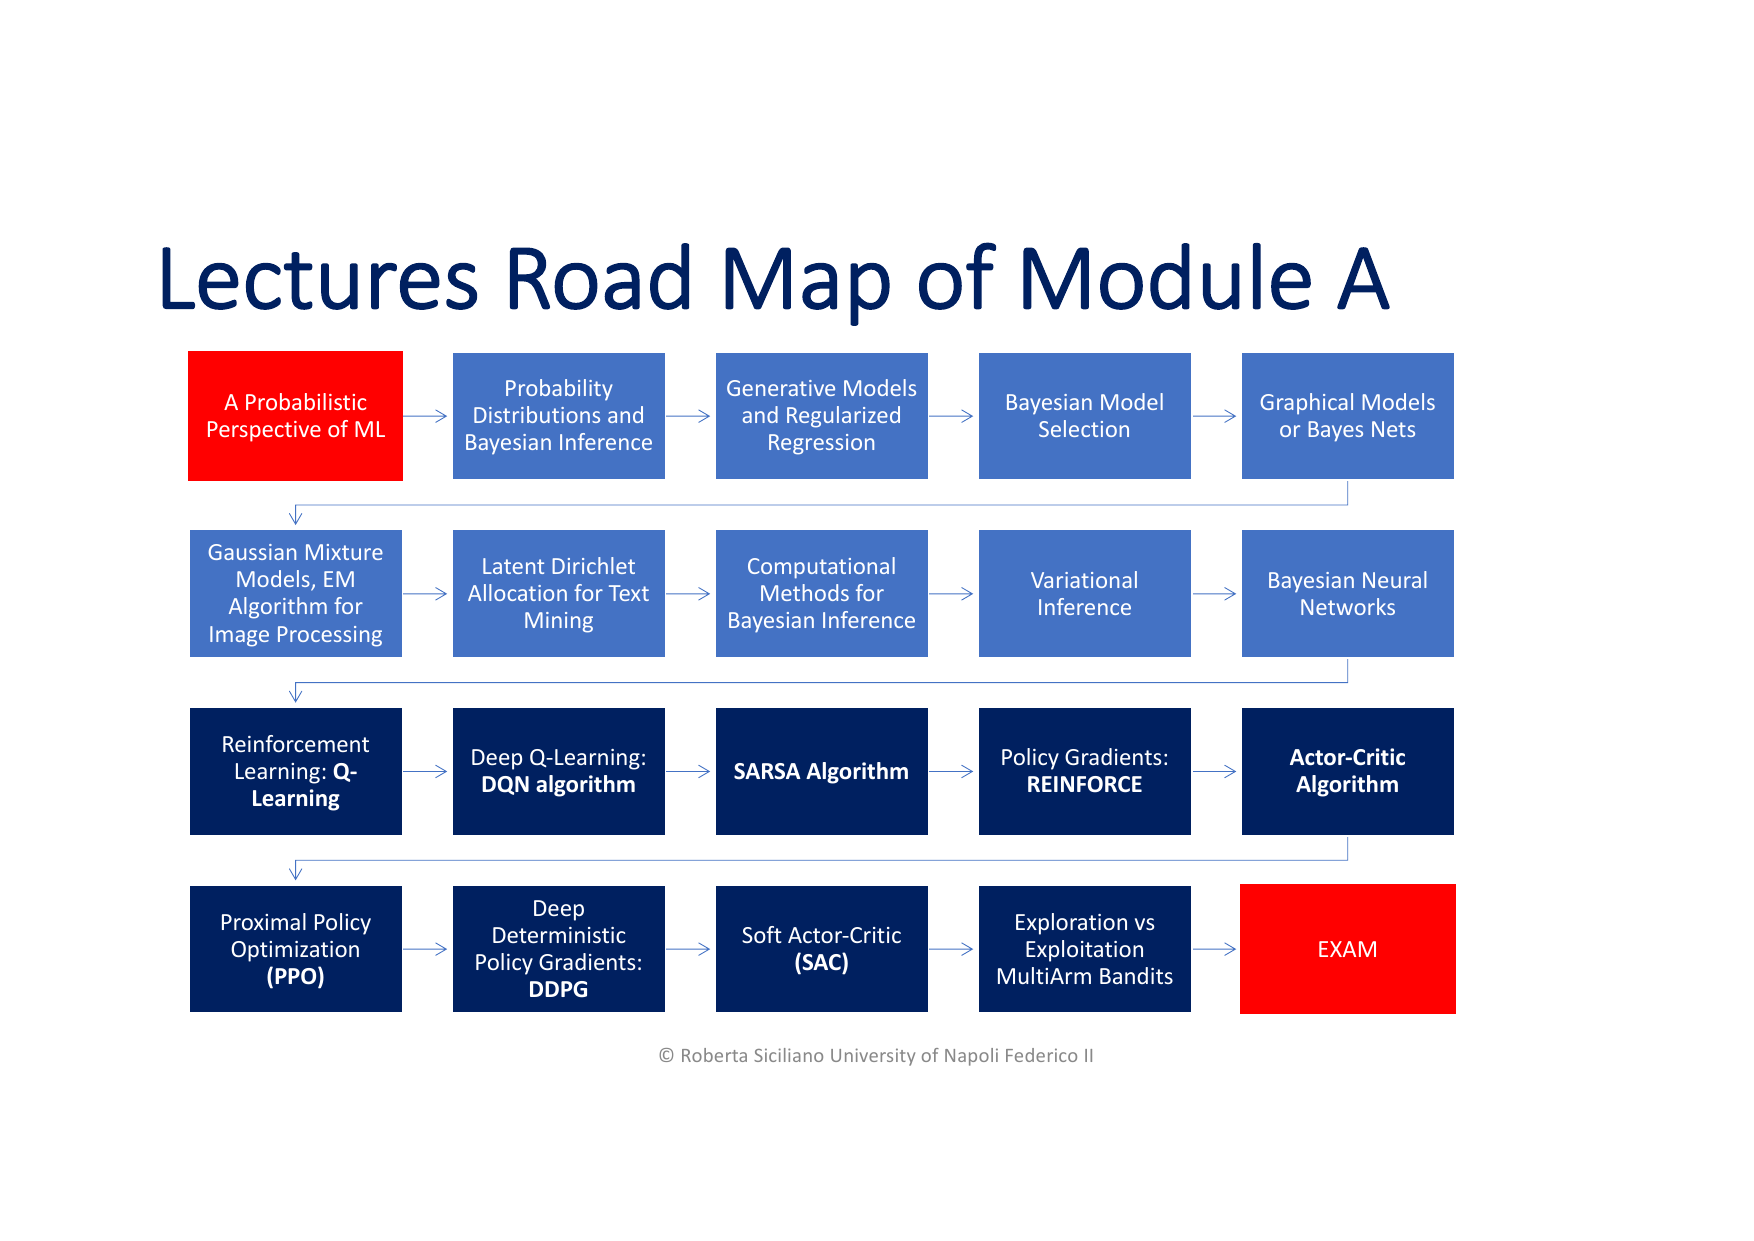
\includegraphics[width=0.85\textwidth]{slide_044}
    \caption{Lectures road map of Module A, from probabilistic ML foundations to advanced Reinforcement Learning algorithms and the exam.}
    \captionsetup{font=footnotesize}
\end{figure}

\subsubsection{Lecture organization and textbooks}

Each lecture combines \textbf{methodology}, \textbf{applications}, and a
\textbf{lab session}. Reference textbooks include Bishop's \textit{Pattern
Recognition and Machine Learning}, Gelman et al.'s \textit{Bayesian Data Analysis},
Murphy's \textit{Probabilistic Machine Learning} series, and -- specifically for
the RL part -- Sutton \& Barto's \textit{Reinforcement Learning: an Introduction}
and Morales' \textit{Grokking Deep Reinforcement Learning}. Scientific articles and
extra material are shared through the course's Team.

\subsubsection{Exam structure}

The exam is based on a \textbf{Portfolio of ASL Projects}, built by completing
assignments during the course (at home or in class); at the exam, this
\textbf{Portfolio of Statistics Projects} is evaluated, and students must also
answer methodological, computational, and application questions.

